%%% The main file. It contains definitions of basic parameters and includes all other parts.

% Meta-data of your thesis (please edit)
\input metadata.tex

% Generate metadata in XMP format for use by the pdfx package
\input xmp.tex

%% Settings for single-side (simplex) printing
% Margins: left 40mm, right 25mm, top and bottom 25mm
% (but beware, LaTeX adds 1in=25.4mm implicitly)
\documentclass[12pt,a4paper]{report}
\setlength\textwidth{145mm}
\setlength\textheight{247mm}
\setlength\oddsidemargin{14.6mm}
\setlength\evensidemargin{14.6mm}
\setlength\topmargin{0mm}
\setlength\headsep{0mm}
\setlength\headheight{0mm}
% \openright makes the following text appear on a right-hand page
\let\openright=\clearpage

%% Settings for two-sided (duplex) printing
% \documentclass[12pt,a4paper,twoside,openright]{report}
% \setlength\textwidth{145mm}
% \setlength\textheight{247mm}
% \setlength\oddsidemargin{14.6mm}
% \setlength\evensidemargin{0mm}
% \setlength\topmargin{0mm}
% \setlength\headsep{0mm}
% \setlength\headheight{0mm}
% \let\openright=\cleardoublepage

%% If the thesis has no printed version, symmetric margins look better
% \documentclass[12pt,a4paper]{report}
% \setlength\textwidth{145mm}
% \setlength\textheight{247mm}
% \setlength\oddsidemargin{7.1mm}
% \setlength\evensidemargin{7.1mm}
% \setlength\topmargin{0mm}
% \setlength\headsep{0mm}
% \setlength\headheight{0mm}
% \let\openright=\clearpage

%% Generate PDF/A-2u
\usepackage[a-2u]{pdfx}

%% Prefer Latin Modern fonts
\usepackage{lmodern}
% If we are not using LuaTeX, we need to set up character encoding:
\usepackage{iftex}
\ifpdftex
\usepackage[utf8]{inputenc}
\usepackage[T1]{fontenc}
\usepackage{textcomp}
\fi

\usepackage{subcaption}

%% Further useful packages (included in most LaTeX distributions)
\usepackage{amsmath}        % extensions for typesetting of math
\usepackage{amsfonts}       % math fonts
\usepackage{amsthm}         % theorems, definitions, etc.
\usepackage{bm}             % boldface symbols (\bm)
\usepackage{booktabs}       % improved horizontal lines in tables
\usepackage{caption}        % custom captions of floating objects
\usepackage{dcolumn}        % improved alignment of table columns
\usepackage{floatrow}       % custom float environments
\usepackage{graphicx}       % embedding of pictures
\usepackage{indentfirst}    % indent the first paragraph of a chapter
\usepackage[nopatch=item]{microtype}   % micro-typographic refinement
\usepackage{paralist}       % improved enumerate and itemize
\usepackage[nottoc]{tocbibind} % makes sure that bibliography and the lists
			    % of figures/tables are included in the table
			    % of contents
\usepackage{xcolor}         % typesetting in color

% The hyperref package for clickable links in PDF and also for storing
% metadata to PDF (including the table of contents).
% Most settings are pre-set by the pdfx package.
\hypersetup{unicode}
\hypersetup{breaklinks=true}

% Packages for computer science theses
\usepackage{algpseudocode}  % part of algorithmicx package
\usepackage{algorithm}
\usepackage{fancyvrb}       % improved verbatim environment
\usepackage{listings}       % pretty-printer of source code

% You might want to use cleveref for references
% \usepackage{cleveref}

% Set up formatting of bibliography (references to literature)
% Details can be adjusted in macros.tex.
%
% BEWARE: Different fields of research and different university departments
% have their own customs regarding bibliography. Consult the bibliography
% format with your supervisor.
%
% The basic format according to the ISO 690 standard with numbered references
\usepackage[natbib,style=iso-numeric,sorting=none]{biblatex}
% ISO 690 with alphanumeric references (abbreviations of authors' names)
%\usepackage[natbib,style=iso-alphabetic]{biblatex}
% ISO 690 with references Author (year)
%\usepackage[natbib,style=iso-authoryear]{biblatex}
%
% Some fields of research prefer a simple format with numbered references
% (sorting=none tells that bibliography should be listed in citation order)
%\usepackage[natbib,style=numeric,sorting=none]{biblatex}
% Numbered references, but [1,2,3,4,5] is compressed to [1-5]
%\usepackage[natbib,style=numeric-comp,sorting=none]{biblatex}
% A simple format with alphanumeric references:
%\usepackage[natbib,style=alphabetic]{biblatex}

% Load the file with bibliography entries
\addbibresource{bibliography.bib}

% Our definitions of macros (see description inside)
\input macros.tex

%%% Title page and various mandatory informational pages
\begin{document}
%%% Title page of the thesis and other mandatory pages

%%% Inscriptions at the opening page of the hard cover

% We usually do not typeset the hard cover, but if you want to do it, change \iffalse to \iftrue
\iffalse

\pagestyle{empty}
\hypersetup{pageanchor=false}
\begin{center}

\large
Charles University

\medskip

Faculty of Mathematics and Physics

\vfill

{\huge\bf\ThesisTypeTitle}

\vfill

{\huge\bf\ThesisTitle\par}

\vfill
\vfill

\hbox to \hsize{\YearSubmitted\hfil \ThesisAuthor}

\end{center}

\newpage\openright
\setcounter{page}{1}

\fi

%%% Title page of the thesis

\pagestyle{empty}
\hypersetup{pageanchor=false}
\begin{center}

\centerline{\mbox{\includegraphics[width=166mm]{img/logo-en.pdf}}}

\vspace{-8mm}
\vfill

{\bf\Large\ThesisTypeTitle}

\vfill

{\LARGE\ThesisAuthor}

\vspace{15mm}

{\LARGE\bfseries\ThesisTitle\par}

\vfill

\Department

\vfill

{
\centerline{\vbox{\halign{\hbox to 0.45\hsize{\hfil #}&\hskip 0.5em\parbox[t]{0.45\hsize}{\raggedright #}\cr
Supervisor of the \ThesisTypeName{} thesis:&\Supervisor \cr
\ifx\ThesisType\TypeRig\else
\noalign{\vspace{2mm}}
Study programme:&\StudyProgramme \cr
\fi
}}}}

\vfill

Prague \YearSubmitted

\end{center}

\newpage

%%% A page with a solemn declaration to the thesis

\openright
\hypersetup{pageanchor=true}
\vglue 0pt plus 1fill

\noindent
I declare that I carried out this \ThesisTypeName{} thesis on my own, and only with the cited
sources, literature and other professional sources.
I understand that my work relates to the rights and obligations under the Act No.~121/2000 Sb.,
the Copyright Act, as amended, in particular the fact that the Charles
University has the right to conclude a license agreement on the use of this
work as a school work pursuant to Section 60 subsection 1 of the Copyright~Act.

\vspace{10mm}

\hbox{\hbox to 0.5\hsize{%
In \hbox to 6em{\dotfill} date \hbox to 6em{\dotfill}
\hss}\hbox to 0.5\hsize{\dotfill\quad}}
\smallskip
\hbox{\hbox to 0.5\hsize{}\hbox to 0.5\hsize{\hfil Author's signature\hfil}}

\vspace{20mm}
\newpage

%%% Dedication

\openright

\noindent
\Dedication

\newpage

%%% Mandatory information page of the thesis

\openright
{\InfoPageFont

\vtop to 0.5\vsize{
\setlength\parindent{0mm}
\setlength\parskip{5mm}

Title:
\ThesisTitle

Author:
\ThesisAuthor

\DeptType:
\Department

Supervisor:
\Supervisor, \SupervisorsDepartment

Abstract:
\Abstract

Keywords:
{\def\sep{\unskip, }\ThesisKeywords}

\vfil
}

% In Czech study programmes, it is mandatory to include Czech meta-data:

\ifx\StudyLanguage\LangCS

\vtop to 0.49\vsize{
\setlength\parindent{0mm}
\setlength\parskip{5mm}

Název práce:
\ThesisTitleCS

Autor:
\ThesisAuthor

\DeptTypeCS:
\DepartmentCS

Vedoucí bakalářské práce:
\Supervisor, \SupervisorsDepartmentCS

Abstrakt:
\AbstractCS

Klíčová slova:
{\def\sep{\unskip, }\ThesisKeywordsCS}

\vfil
}

\fi

}

\newpage

%%% Further pages will be numbered
\pagestyle{plain}


%%% A page with automatically generated table of contents of the thesis

\tableofcontents

%%% Each chapter is kept in a separate file
\chapter*{Introduction}
\addcontentsline{toc}{chapter}{Introduction}

In recent years, mobile technologies have advanced rapidly, which had a significant impact on various aspects of our lives, especially in education and culture. Museums, for example, are now introducing mobile technologies to increase visitor engagement and learning experiences. Traditional museum tours are often based on static information stands and guided tours, which may not match the pace and preferences of individual visitors. To solve this problem, we propose a mobile application that uses real-time image classification to create an interactive and personalized museum guide.

The core of this application is a fine-tuned MobileNet neural network converted to TensorFlow Lite for efficient image classification on mobile devices. The model has been trained on a dataset with frames extracted from videos of museum exhibits. 

Users of the application need to point the camera of their mobile device at the exhibit. The app will automatically take pictures at regular intervals and classify them into one of several predefined categories. After successful classification, the application extracts detailed information about the exhibit from a local database and displays it to the user. This process turns a museum visit into an interactive process where information is easily accessible.

The development of this application included several key steps: video recording and frame extraction, model training and fine-tuning, Android application development and model integration into this application. Each stage presented unique tasks and required special technical solutions, which are discussed in detail in this paper.

The main goal of this project is to demonstrate how mobile image classification can improve the experience of museum visitors. By automating the process of information recognition and retrieval, the application reduces the need for physical guides and static information boards, allowing visitors to explore exhibits at their own pace and according to their interests.

In conclusion, this work aims to provide a comprehensive report on the development and implementation of a mobile application for real-time image classification of museum exhibits. It highlights the technical and practical aspects, as well as the potential benefits for museums and their visitors. Through this work, we hope to contribute to the ongoing efforts to integrate technology into the cultural and educational context, making learning more accessible and fun.
\chapter{Related Work}

With the advent of mobile technology, museums are exploring new ways to increase visitor engagement in the learning process. Mobile applications and interactive guides are being used to conduct personalized tours, receive information in augmented reality, and more.

\section*{Mobile Applications in Museums}

Several projects have demonstrated the potential of mobile applications to improve the museum experience. For example, the development of mobile applications such as the ``Louvre Visit, Tours \& Guide`` \cite{louvre_app} and the ``British Museum Audio`` \cite{british_museum_app} has shown that visitors can benefit from access to a digital guidebook that not only provides additional information about the exhibits, but also shares practical information, navigation, and flexible self-guided tours.

However, to access information, these applications mainly use manual user input, such as scanning QR codes or entering exhibit numbers. Despite its effectiveness, this approach lacks the speed and seamlessness that can be achieved with more advanced technologies such as image recognition and real-time classification.

\section*{Image Classification in Cultural Heritage Institutions}

The integration of image recognition technology into museum applications represents a significant step forward in creating a more interactive and responsive user experience. For example, a project called ``CHESS`` (Cultural Heritage Experiences through Socio-personal interactions and Storytelling) \cite{chess_project}, co-funded by the European Commission, has explored the use of image recognition to identify works of art and provide augmented reality experience. Such systems allow visitors to point their devices at the exhibits to instantly receive detailed information, thereby improving the learning process by minimizing the effort required to interact with the content.

\section*{Summary}

In summary, the integration of mobile applications and image recognition models into the museum experience has demonstrated great potential in increasing visitor engagement and learning. While traditional mobile guides provide valuable information, the addition of real-time image classification represents a significant step forward in providing seamless interaction. As museums continue to introduce these technologies, visitors' experiences are likely to become more personalized, dynamic, and informative.
\chapter{Theoretical Background}

\section{Convolutional Neural Networks (CNNs)}

\subsection{Introduction to CNNs}

Convolutional Neural Networks (CNNs) are a class of deep learning models that have gained widespread popularity due to their ability to effectively analyze visual data. Originally inspired by the organization of the animal visual cortex, CNNs are a perfect tool for image recognition tasks.

A distinctive feature of CNNs is their ability to capture local dependencies in images using convolutional layers. These layers apply trainable filters (or kernels) over the input image to detect various features such as edges, textures, and patterns. As the network deepens, it gradually captures more complex and abstract features, which allows for highly accurate image classification.

\subsection{Architecture of CNNs}

A typical CNN architecture consists of several key components: an input layer, convolutional layers, pooling layers, and fully connected layers. Each component plays a specific role in processing the input data and contributing to the overall functionality of the network.

\begin{figure}[h]
    \centering
    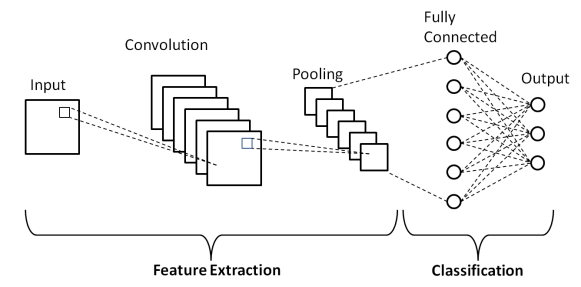
\includegraphics[width=0.7\textwidth]{img/cnn-architecture.png}
    \caption{Illustration of a CNN architecture. Source: \href{https://www.researchgate.net/publication/336805909_A_High-Accuracy_Model_Average_Ensemble_of_Convolutional_Neural_Networks_for_Classification_of_Cloud_Image_Patches_on_Small_Datasets}{ResearchGate article.}}
    \label{fig:cnn-architecture}
\end{figure}

\subsubsection{Convolutional Layers}

Convolutional layers are the main building block of a CNN architecture. They apply a set of filters over the input image, where each filter slides (or convolves) across the image to produce a feature map. This operation helps the network learn spatial hierarchies of features, where earlier layers might detect simple edges or textures, and deeper layers capture more complex structures like shapes or even entire objects.

The mathematical operation behind convolution involves multiplying each filter's weights by the corresponding pixel values in the input image and summing the results. This process is repeated as the filter moves across the image, resulting in a feature map that highlights the presence of the feature detected by the filter.

Mathematically, the convolution operation for a single filter can be expressed as:

\[
\text{FeatureMap}(i,j) = \sum_{m,n} I_{i-m,j-n} W_{m,n} + b
\]

where \(W\) represents the filter weights, \(I\) represents the input image pixel values, and \(b\) is the bias term.

\subsubsection{Activation Functions}

After convolution, the output feature map is passed through a non-linear activation function, typically the Rectified Linear Unit (ReLU). The ReLU activation function is defined as:

\[
ReLU(x) = \max(0, x)
\]

ReLU introduces non-linearity into the model, which is needed in order to learn more complex patterns in the data. Other activation functions, for example hyperbolic tangent (tanh), can also be used, but ReLU is preferred in most CNN architectures due to its simplicity and effectiveness in avoiding the vanishing gradient problem.

\subsubsection{Pooling Layers}

Pooling layers, often placed between consecutive convolutional layers, are used to reduce the dimensions of the feature maps. This operation reduces the network's computational complexity and makes the learned features more invariant to small translations of the input image.

The most common pooling operation is max pooling, which selects the maximum value from each region of the feature map. The formula for max pooling over a 2x2 region is:

\[
\text{MaxPool}(i,j) = \max \{ I_{2i,2j}, I_{2i,2j+1}, I_{2i+1,2j}, I_{2i+1,2j+1} \}
\]

Another popular type of pooling operation is average pooling, which computes the region's average value instead of the maximum.

Overall, pooling layers gradually reduce the spatial size of the image representation, making the network more efficient while retaining the most important features. 

\subsubsection{Fully Connected Layers}

After several convolutional and pooling layers, the resulting feature maps are flattened into a one-dimensional vector to be processed by one or more fully connected layers. These layers function like a standard neural network, where each neuron is linked to every neuron in the next layer. Finally, the last fully connected layer, called the output layer, performs the final classification.

The CNN's output layer typically uses a softmax activation function for multi-class classification tasks. The softmax function converts the output scores into probabilities, allowing the network to assign a class label to the input image.

\subsection{Conclusion}

CNNs have been successfully used to solve various image classification tasks, including object detection, face recognition, and medical image analysis. In the context of museum applications, CNNs are used to classify and recognize various types of exhibits, ranging from paintings and sculptures to historical artifacts. By fine-tuning pre-trained CNN models on museum-specific datasets, it is possible to achieve high accuracy in identifying exhibits, thereby enhancing the visitor experience.

\section{MobileNet}

MobileNet is a class of efficient convolutional neural networks specifically designed for mobile and embedded vision applications. Introduced by Howard et al. \cite{howard_mobilenet}, MobileNet addresses the need for high-performance neural networks that can work efficiently on devices with limited resources (e.g., smartphones).

\subsection{Architecture of MobileNet}

The core innovation of MobileNet is the use of depthwise separable convolutions, which break down the standard convolution operation into two simpler steps: depthwise convolution (applying a single filter per input channel) and pointwise convolution (combining the output channels). This approach significantly reduces the number of calculations (23x fewer multiplications for an 8x8x3 image) and model size, making MobileNet fast and lightweight.

\begin{figure}[h]
    \centering
    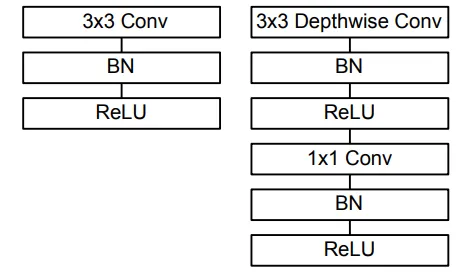
\includegraphics[width=0.7\textwidth]{img/mobilenet.png}
    \caption{Left: Standard Convolutional layer, Right: Depthwise Separable Convolutional layers in MobileNet. Source: image from the original paper.}
    \label{fig:mobilenet}
\end{figure}

\subsection{MobileNet Versions}

There are three versions of the MobileNet architecture, each improving upon the last in terms of efficiency and accuracy:

\textbf{MobileNetV1} was the first iteration, known for being ten times faster and smaller than the VGG16 architecture, making it a popular choice for mobile applications due to its significant reduction in computational resources \cite{pandrii_mobilenet}.

\textbf{MobileNetV2} introduced inverted residual blocks with linear bottlenecks, which enhanced the model's ability to learn more efficient representations. This version is approximately 30\% smaller and 0.3 times faster than MobileNetV1 while being 1\% more accurate \cite{pandrii_mobilenet}.

\textbf{MobileNetV3} builds upon the improvements of V2 by incorporating advances such as Neural Architecture Search (NAS) and Squeeze-and-Excitation (SE) modules. MobileNetV3 is twice as fast and 30\% smaller than V2 but with a slight trade-off in accuracy, being 3\% less accurate than MobileNetV2 \cite{pandrii_mobilenet}.

\textbf{Note on Model Choice:} Despite the improvements in MobileNetV3, MobileNetV2 was chosen for this thesis due to its optimal balance between accuracy and efficiency. While V3 offers better speed and smaller size, the slight reduction in accuracy was not suitable for the high accuracy requirements of this project.

\subsection{Conclusion}

Thanks to its efficient design, MobileNet offers a well-balanced architecture ideal for real-time applications on mobile devices. In this thesis, MobileNet's lightweight structure is crucial for effectively and accurately classifying museum exhibits, providing visitors with enhanced learning experiences while maintaining optimal performance on mobile hardware.

\section{Transfer Learning}

\subsection{Introduction to Transfer Learning}

Transfer learning is a machine learning technique of using knowledge gained during the execution of one task to improve the performance of another related task. Instead of building and training a new model from scratch, scientists and engineers can use pre-trained models as a starting point, reducing the need for large amounts of data and computational resources.

In traditional machine learning, models are usually trained from scratch using a large dataset for a specific task. This process involves learning feature representations from the raw data, which can be time-consuming and computationally intensive. However, the early layers of neural networks often learn general features like edges and textures that are useful across tasks, so transfer learning takes advantage of these general features by reusing the early layers of a pre-trained model and fine-tuning the later layers on the target task. The most common approach to transfer learning involves:

1. \textbf{Pre-training:} A model is first trained on a large source dataset with extensive labeled examples (e.g., ImageNet). During this phase, the model learns to extract general features from the input data.

2. \textbf{Fine-tuning:} The pre-trained model is then adapted to the target task by continuing training on a smaller, task-specific dataset. This process fine-tunes the model's weights to better fit the characteristics of the target data while retaining the knowledge acquired during pre-training.

\subsection{Transfer Learning in CNNs}

Transfer learning is widely used in the context of CNNs, especially for image classification tasks. During transfer learning, the early layers of a pre-trained CNN are often frozen (i.e., their weights are kept constant), and only the deeper layers are fine-tuned. This approach keeps the general feature extraction capabilities of the early layers, which are often relevant across different tasks, while adapting the model to the specific characteristics of the target data.

\subsection{Transfer Learning in Museum Exhibit Classification}

In the context of museum exhibit classification, transfer learning is beneficial due to the limited availability of labeled data for training. Museum exhibits vary widely in style, material, and content, making it difficult to compile a comprehensive dataset. By using a pre-trained CNN model like MobileNet, which has been trained on a large, diverse dataset such as ImageNet, it is possible to effectively classify museum exhibits with a smaller, domain-specific dataset.

\subsection{Conclusion}

Transfer learning enables the reuse of pre-trained models to solve new tasks with limited data and resources. In this thesis, transfer learning is crucial for developing an efficient and accurate model for museum exhibit classification, ensuring high-quality performance on mobile devices.
\chapter{Model Training}\label{chapter:model_training}

\section{Data Collection}

The first step in the model training process involved preparing the dataset for training. This was achieved by recording a video of each exhibit in the museum and extracting frames from these videos. The video recordings were made using a smartphone camera, capturing various angles to ensure that users will get correct results from various angles as well. To avoid class imbalance, the number of frames to extract was determined based on the shortest video in the dataset, and the frames were then extracted at regular intervals using the \texttt{ffmpeg} tool. The extracted frames were saved in a directory structure, with each exhibit's frames stored in a separate folder under \texttt{res/frames/}. The frames were named sequentially (e.g., \texttt{frame\_01.jpg}). The corresponding code can be found in the \texttt{extract\_frames.py} script.

Additional information about each exhibit, such as the exhibit ID, title, author, and date period, was stored in a CSV file named \texttt{upm\_exhibits\_dataset.csv}. This metadata was used to label the frames during the training process (with the corresponding ID of each exhibit) and display information about the exhibits in the mobile application.

\section{Explored Solutions}

We explored two main approaches to solve the problem of exhibit recognition: embedding-based similarity search and direct classification using transfer learning.

\subsection{Embedding-based Similarity Search}

The first approach involved using a neural network to generate image embeddings. An embedding is a numeric vector representation capturing essential visual features of each image. The core idea was to pre-compute embeddings for all exhibit images in the training dataset. During inference, the neural network would generate an embedding for the user's input image, and the application would then perform a similarity search against stored embeddings to identify the closest match.

The primary advantage of this method is flexibility: adding new exhibits would not require retraining the neural network from scratch. Instead, only new embeddings would need to be generated and added to the existing collection, significantly simplifying updates.

However, this approach presented several practical challenges:

\begin{itemize}
    \item \textbf{Storage Constraints}: Our application is designed for offline usage within the museum, so image embeddings must be stored on the mobile device. Mobile devices have limited storage capacity. Storing embeddings for each exhibit --- especially as the museum collection expands --- could quickly become impractical due to the sheer volume of data.
    \item \textbf{Computational Efficiency}: Performing real-time similarity searches is computationally demanding on mobile hardware, which could lead to performance issues, especially with larger datasets.
\end{itemize}

These considerations led us to evaluate alternative methods better suited for mobile deployment and offline operation.

\subsection{Transfer Learning with Direct Classification}

The second approach, ultimately selected, was transfer learning for direct image classification. This method fine-tuned a pre-trained convolutional neural network to classify our museum exhibits. The network directly outputs probabilities corresponding to each exhibit class, eliminating the need for similarity searches.

This method offers several significant advantages:

\begin{itemize}
    \item \textbf{Efficiency and Speed}: Direct classification is computationally efficient and provides quick predictions suitable for real-time recognition on mobile devices.
    \item \textbf{Simplified Integration}: Only a single, optimized TensorFlow Lite model must be stored on the device, significantly reducing storage overhead and simplifying the integration process.
\end{itemize}

However, this approach comes with the following trade-off: when new exhibits are introduced, the model must be retrained to include these additional classes. Nonetheless, this issue can be solved by automating the training pipeline, as training times with transfer learning are typically short.

Considering these factors, direct classification using transfer learning was selected as the most suitable solution due to its balance between accuracy, performance, storage efficiency, and ease of integration.

\section{Model Selection and Setup}

As already mentioned, transfer learning was employed to adapt the pre-trained model to our task of classifying museum exhibits. This approach leverages the general features learned from pre-training and fine-tunes the chosen model to recognize the unique characteristics of the specific data. More information on transfer learning can be found in Section~\ref{section:transfer_learning}.

For our task, the MobileNetV2 architecture was selected as the base model. MobileNetV2 is a lightweight convolutional neural network specifically designed for mobile applications. It balances efficiency and accuracy, making it ideal for real-time image classification tasks on resource-constrained devices like smartphones. Further details on MobileNetV2 can be found in Section~\ref{section:mobilenet}.

The transfer learning setup involved the following steps:

\begin{enumerate}
   \item \textbf{Freezing Pre-trained Layers:} The pre-trained MobileNetV2 model was loaded with its convolutional base set to non-trainable. By freezing the early layers, the model retained its ability to extract general features learned from ImageNet, for example, detect edges, textures, and shapes.
   
   \item \textbf{Adding Custom Layers:} Custom layers were added on top of the frozen layers to adapt the model to our dataset. These included:
   \begin{itemize}
       \item \textbf{Global Average Pooling:} To reduce spatial dimensions of feature maps to a single vector per feature map, summarizing the important information.
       \item \textbf{Dense Layer:} A fully connected layer with 1024 units and ReLU activation to learn complex feature combinations relevant for exhibit classification.
       \item \textbf{Dropout Layer:} Included with a rate of 0.1 to prevent overfitting by randomly setting a fraction of input units to zero during training.
       \item \textbf{Output Layer:} A dense layer with softmax activation, where the number of units corresponds to the number of exhibit classes. This layer outputs predicted probabilities for each class.
   \end{itemize}
\end{enumerate}

\section{Training Process}

In the beginning, it is important to note that many aspects of training a neural network --- such as model architecture, learning rates, batch size, or number of epochs --- are typically determined through experimentation. While there are commonly accepted starting points (e.g., using a batch size of 16 or 32, or the Adam optimizer with a standard learning rate), there is no one-size-fits-all configuration. Each dataset and task is different, and therefore requires iterative testing and tuning to find the combination of parameters that gives the best performance. In this project, several choices were made based on such experimentation.

Also, as part of the experimentation process, the training process was divided into two main phases: initial training, in which only the custom layers were trained, and additional fine-tuning, where some of the pre-trained layers were unfrozen to allow for further learning on the museum exhibit dataset.

\subsection{Initial Training and Evaluation}

During the initial training phase, the custom layers added on top of the pre-trained base were trained on the museum exhibit dataset. The training setup and details are as follows:

\begin{itemize}
   \item \textbf{Optimizer:} Adam optimizer, used with the default learning rate of \(1 \times 10^{-3}\).
   \item \textbf{Loss Function:} Categorical cross-entropy, suitable for multi-class classification.
   \item \textbf{Metrics:} Accuracy, showing how often the predictions matched actual labels.
   \item \textbf{Epochs:} 20 epochs, determined by monitoring the model's performance on the validation set (will be covered later in this section).
   \item \textbf{Batch Size:} Batch size of 16, which is a common choice.
   \item \textbf{Validation:} 20\% of the data was kept aside to monitor how well the model performed on unseen data.
\end{itemize}

This setup gives us 0.945 accuracy on the validation set after 20 epochs of training, and it can be seen in Figure~\ref{fig:initial_training} that there is no significant improvement in accuracy after the 10th epoch, indicating that the model has likely converged (same results were obtained when training for 40 epochs).

\begin{figure}[h]
    \centering
    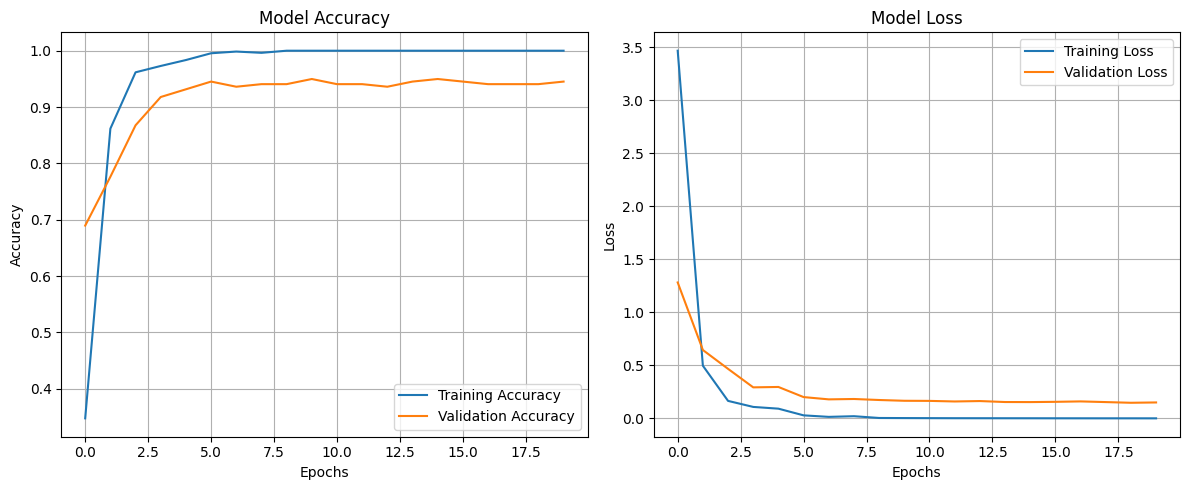
\includegraphics[width=1.0\textwidth]{img/initial-training.png}
    \caption{Training and validation accuracy and loss during the initial training phase.}\label{fig:initial_training}
\end{figure}

While the initial results are already quite good, further fine-tuning might improve the model's performance by adjusting some of the pre-trained layers to better fit the new dataset.

\subsection{Additional Fine-tuning and Evaluation}

After the initial training, the model was trained further with some of the pre-trained layers unfrozen. This optional step can improve the model's performance by adjusting some of the pre-trained layers to better fit the new dataset.

The number of layers to unfreeze depends on how similar the new dataset is to the dataset the model was initially trained on (ImageNet) and on the size of the new dataset. If the new data is very different, unfreezing more layers can help the model adjust better. As for the size, if the new dataset is small, unfreezing too many layers can lead to overfitting. A common strategy is to unfreeze the last few dozen layers. For example, the official TensorFlow tutorial~\cite{tensorflow_transfer_learning} demonstrates unfreezing MobileNetV2 from about layer 100 onward (out of 154) --- i.e., fine-tuning the last 54 layers (around the top one-third of the network). It is also recommended to fine-tune with a lower learning rate, since large weight updates on pre-trained layers can disrupt the learned features, leading to worse performance.

We experimented with unfreezing the last 14, 24, and 34 layers of the pre-trained model. During fine-tuning, the learning rate was lowered to \(1 \times 10^{-5}\) to avoid significant changes to already learned features. Fine-tuning continued for another 20 epochs after the initial training. The best results were achieved when unfreezing the last 34 layers (meaning that the first 120 layers were frozen), which resulted in a validation accuracy of 0.959 after fine-tuning. This gives us a 1.4\% improvement over the initial training phase, which is a slight improvement considering that the model was already performing well. The results of the fine-tuning phase can be seen in Figure~\ref{fig:fine_tuning}.

\begin{figure}[h]
    \centering
    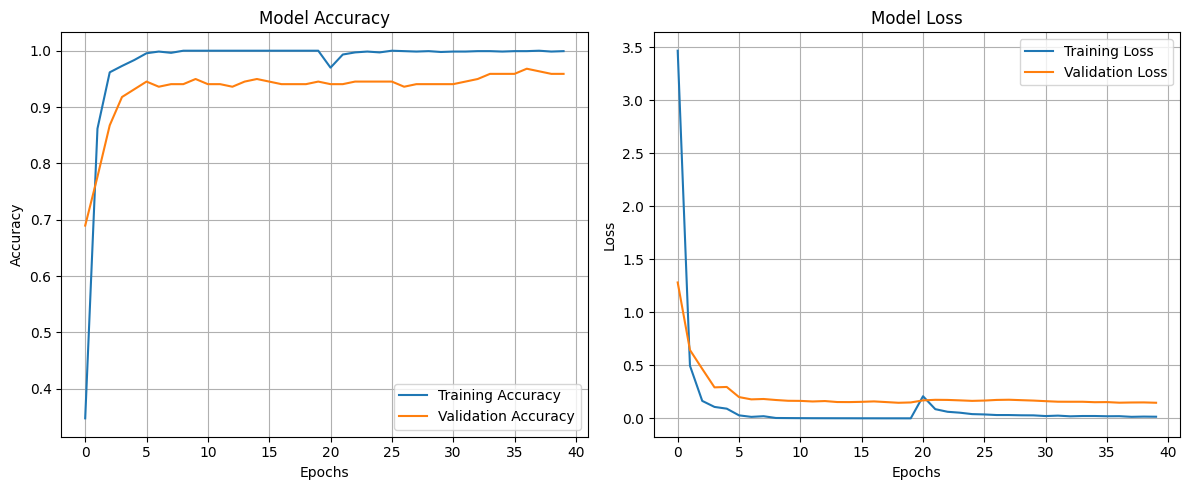
\includegraphics[width=1.0\textwidth]{img/fine-tuning.png}
    \caption{Training and validation accuracy and loss during the fine-tuning phase.}\label{fig:fine_tuning}
\end{figure}

\section{Other Experiments}

Several other experiments were conducted during the training process to explore different configurations and their impact on model performance. These included:

\begin{itemize}
    \item \textbf{Batch Sizes:} Different batch sizes (8, 16, and 32) were tested, which did not affect the model's performance. A batch size of 16 was chosen as a good compromise between training speed and memory usage.
    \item \textbf{Data Augmentation:} Various data augmentation techniques were applied, such as rotation, width and height shifts, and zooming. However, these did not improve the model's performance; instead, they increased training time. Therefore, no data augmentation was used in the final model.
    \item \textbf{More Layers}: Additional dense layers were added to the model, which increased the model's training time but did not improve the accuracy.
    \item \textbf{Increased Dropout Rate:} The dropout rate was increased to 0.5, which resulted in a lower validation accuracy.
\end{itemize}

Thus, the final model configuration was chosen based on the best results from these experiments, which included a batch size of 16, no data augmentation, one dense layer, and a dropout rate of 0.1.

In the following section, we will analyze the misclassifications made by the model during the validation phase to better understand its performance and identify potential areas for improvement.

\section{Analysis of Misclassifications}

To better understand the model's performance, we analyzed the misclassifications made during the validation phase. This analysis helps identify patterns in errors and provides insights into potential improvements.

Of 219 images in the validation set, nine were misclassified, resulting in a validation accuracy of 0.959. In Figure~\ref{fig:misclassifications}, we can see the misclassified images along with their actual and predicted labels. Actual labels are shown in the second column, while the model's predictions are in the third column.

\begin{figure}[h]
    \centering
    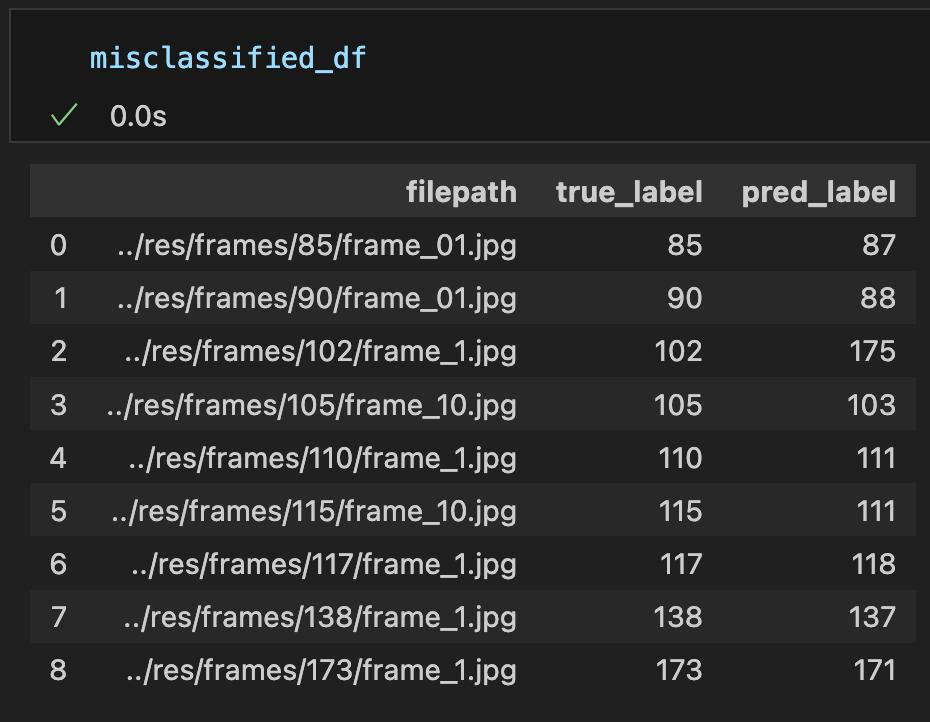
\includegraphics[width=0.7\textwidth]{img/misclassifications.png}
    \caption{Misclassified images with their true labels and model predictions.}\label{fig:misclassifications}
\end{figure}

If we look at the actual labels and predicted labels, we can see that most of them are very close to each other (85--87, 90--88, 105--103, and so on). Exhibits were recorded and labeled one after another, so the exhibits whose labels are close to each other are likely to be visually similar, because they are from the same collection or share the same style or theme. Moreover, some frames from video recordings contain multiple exhibits, which can lead to confusion for the model. For example, the image with label 138 contains two exhibits (with a true label 138 and our predicted label 137) in the same frame, which makes it difficult for the model to distinguish between them. Figure~\ref{fig:misclassifications_examples1} and Figure~\ref{fig:misclassifications_examples2} show some examples of misclassified images with their true labels and model predictions.

This leads us to the conclusion that the model is performing well enough for the exhibits that are visually distinct, but it might struggle with similar-looking exhibits or those captured in the same frame. In order to address this issue, our application will provide the user with the top-recognized exhibit as the main prediction, and up to four alternatives for user selection ordered by confidence level. This approach will help improve the user experience and ensure that users can find the information they are looking for, even if the model makes a mistake.

\begin{figure}[h]
    \centering

    \begin{subfigure}[b]{0.4\textwidth}
        \centering
        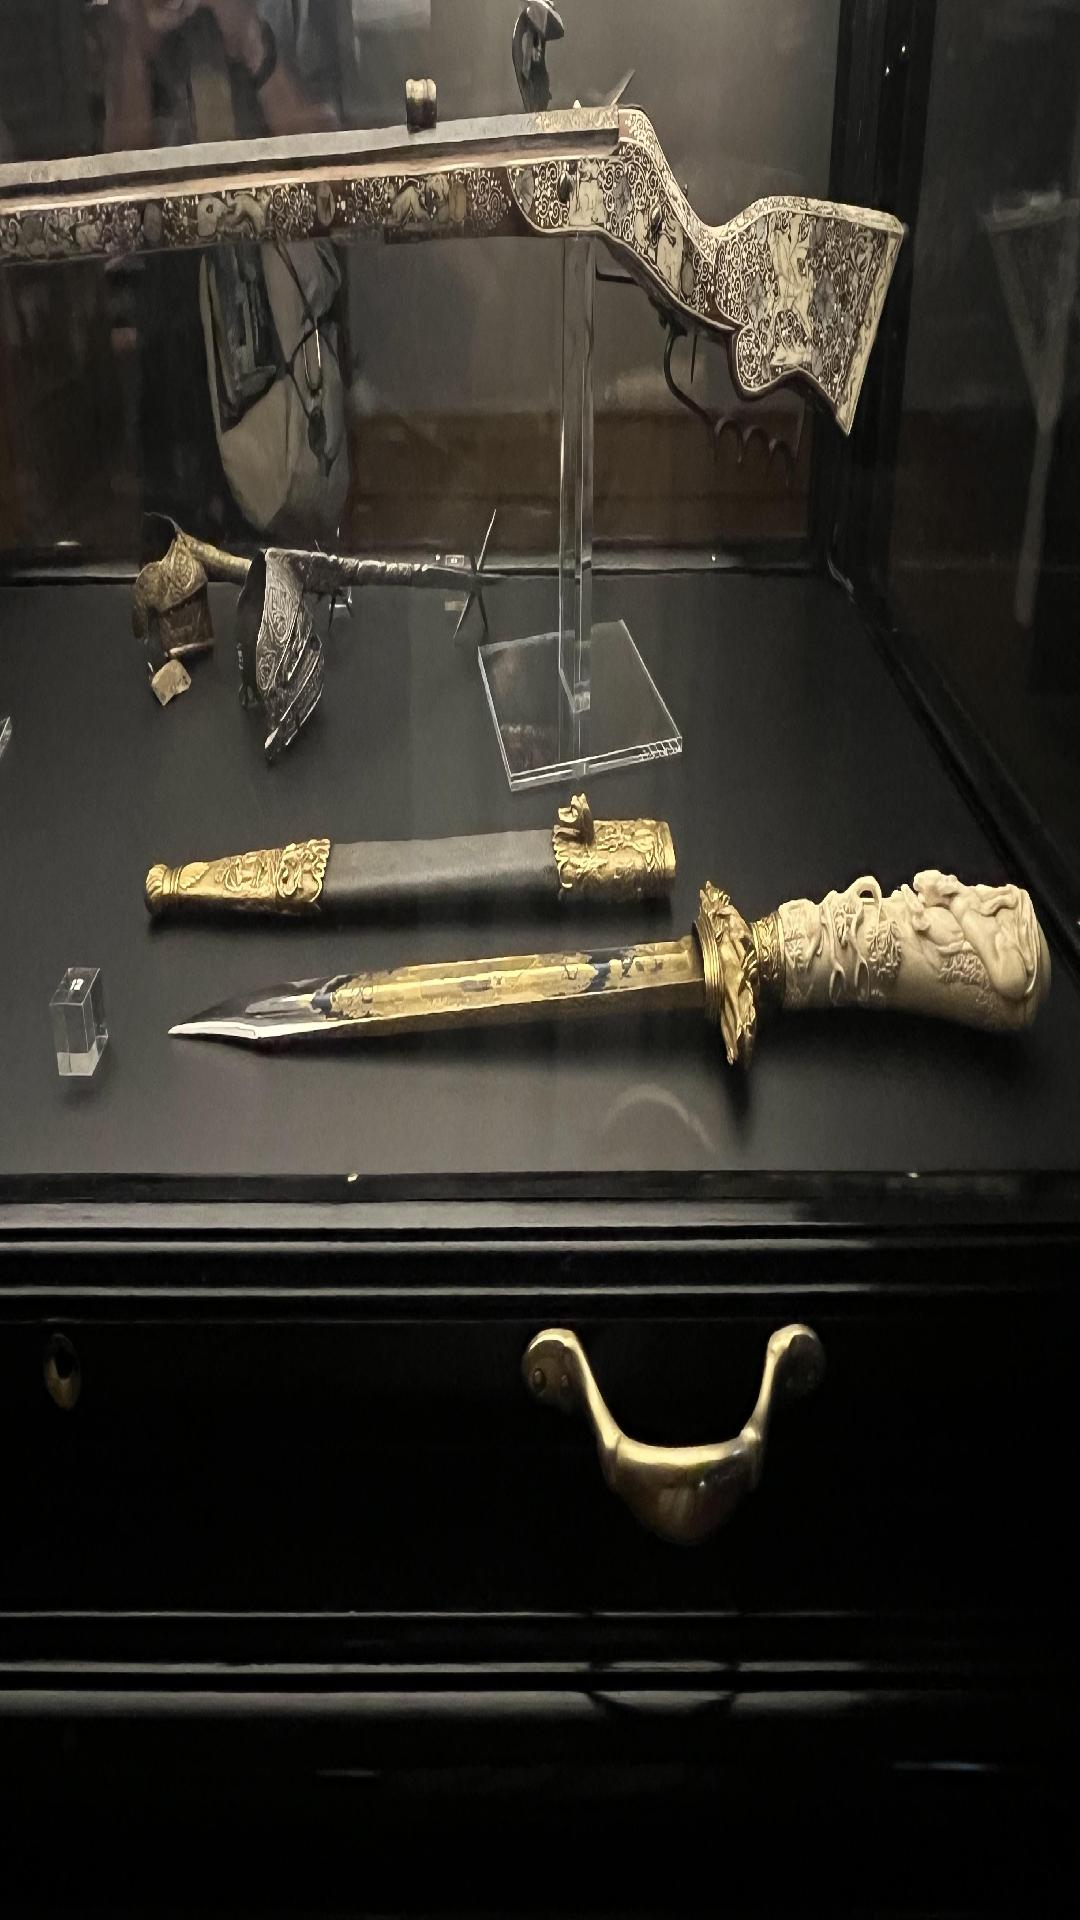
\includegraphics[width=\textwidth]{img/138.jpg}
        \caption{Input image with true label 138.}
    \end{subfigure}
    \hfill
    \begin{subfigure}[b]{0.4\textwidth}
        \centering
        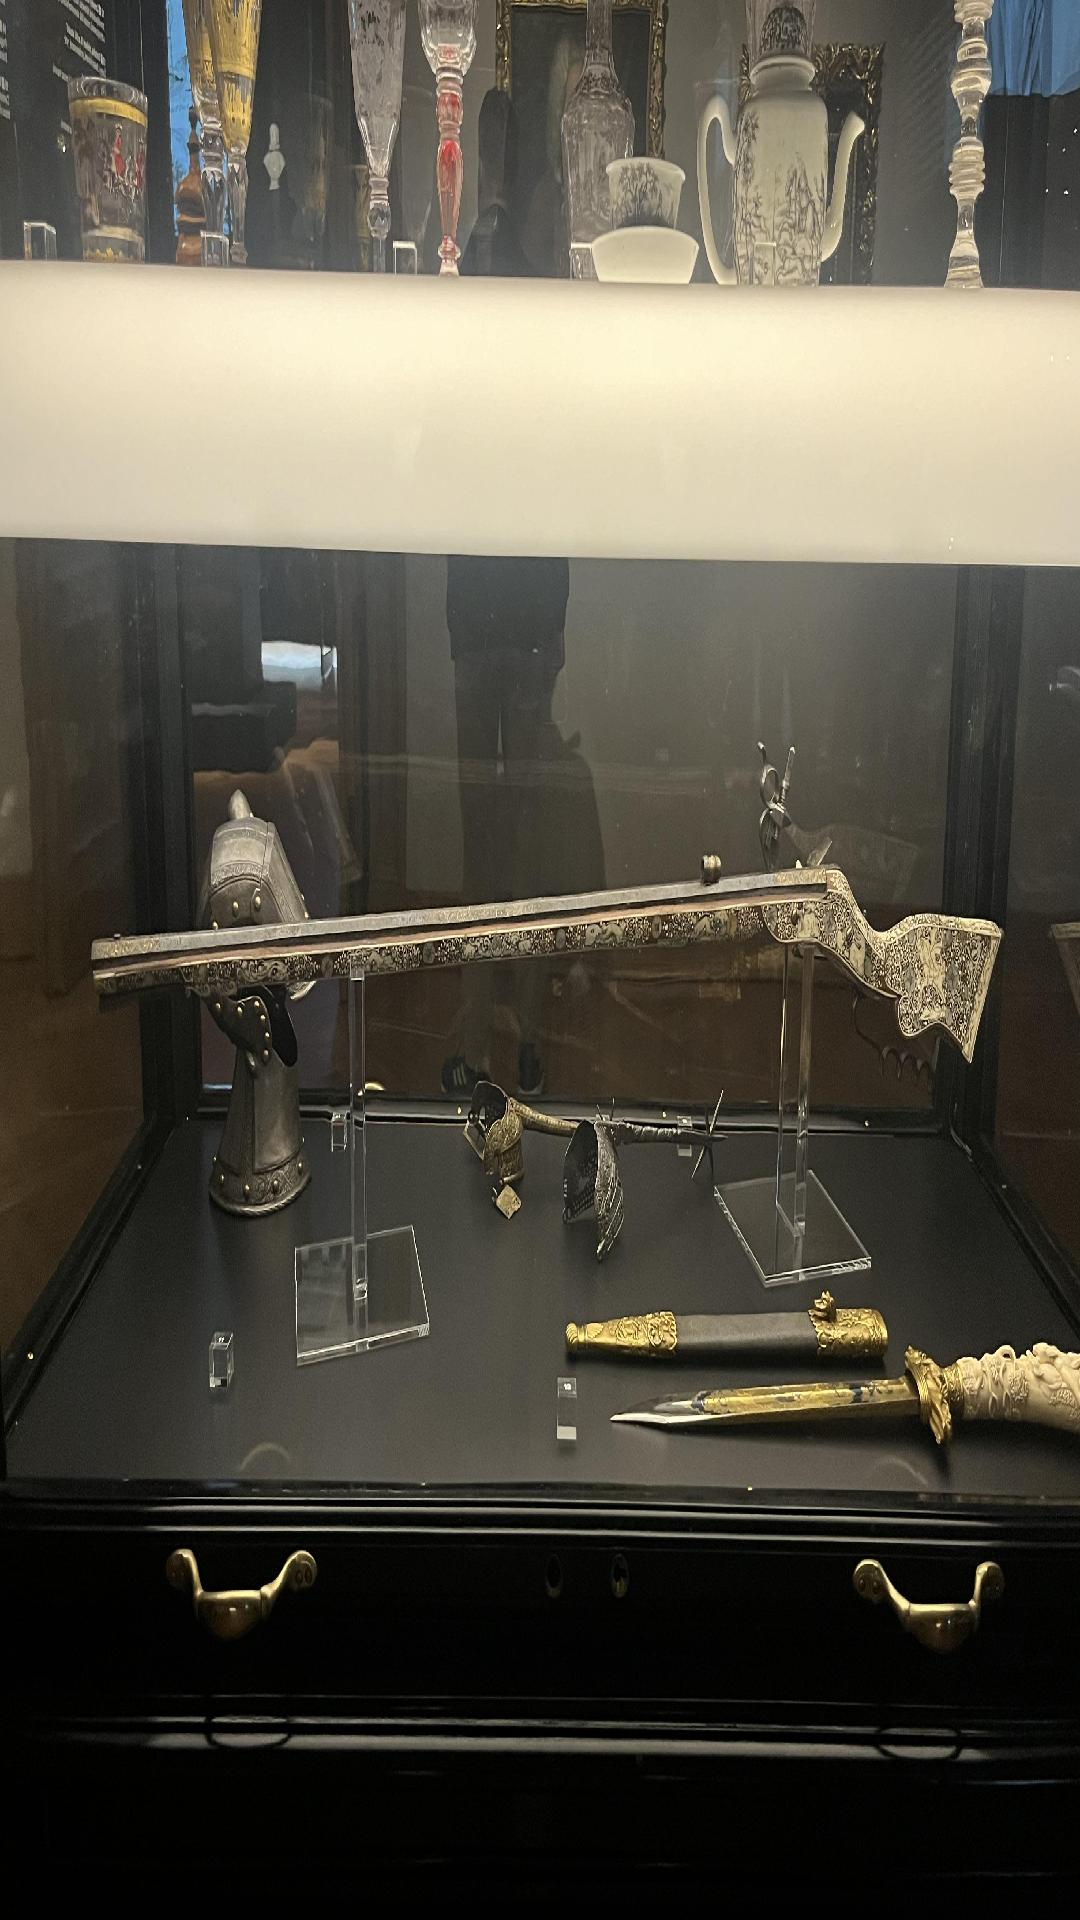
\includegraphics[width=\textwidth]{img/137.jpg}
        \caption{Image of the predicted label 137.}
    \end{subfigure}

    \vspace{1em}

    \begin{subfigure}[b]{0.4\textwidth}
        \centering
        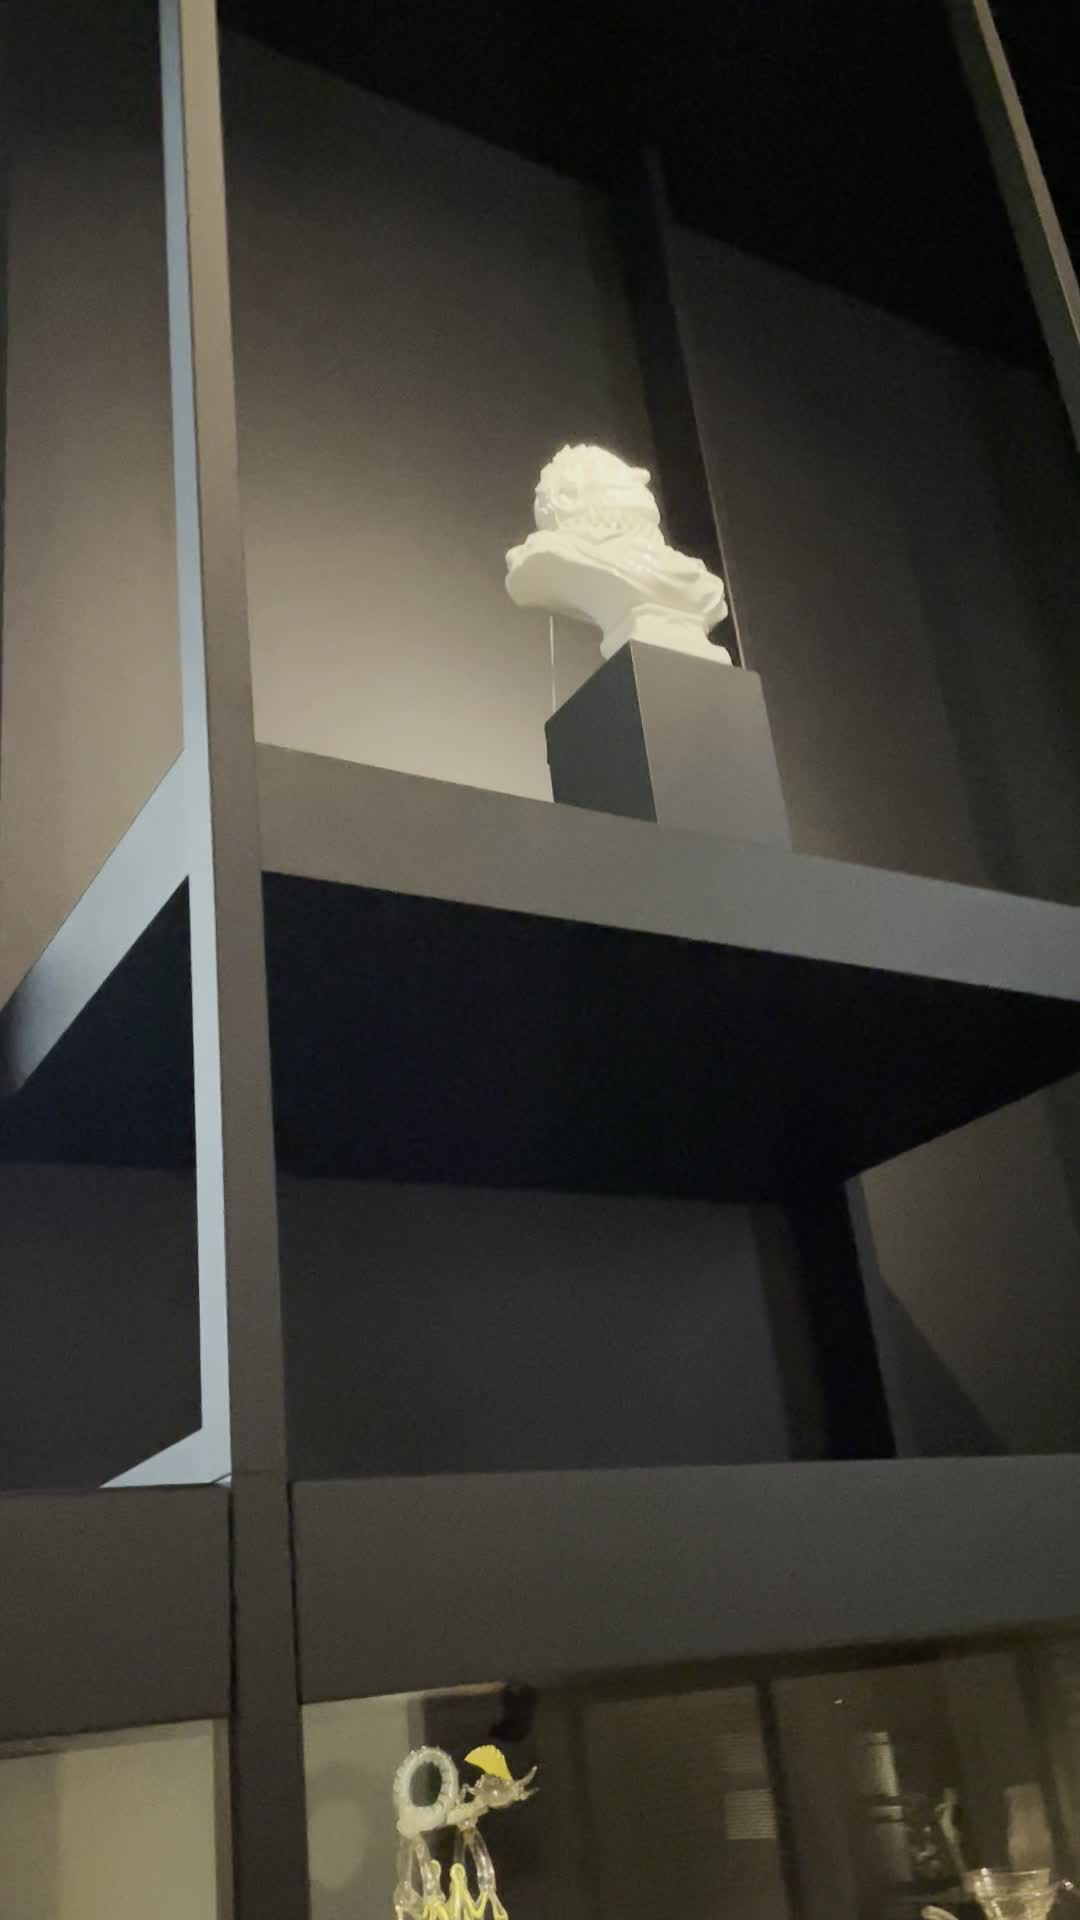
\includegraphics[width=\textwidth]{img/85.jpg}
        \caption{Input image with true label 85.}
    \end{subfigure}
    \hfill
    \begin{subfigure}[b]{0.4\textwidth}
        \centering
        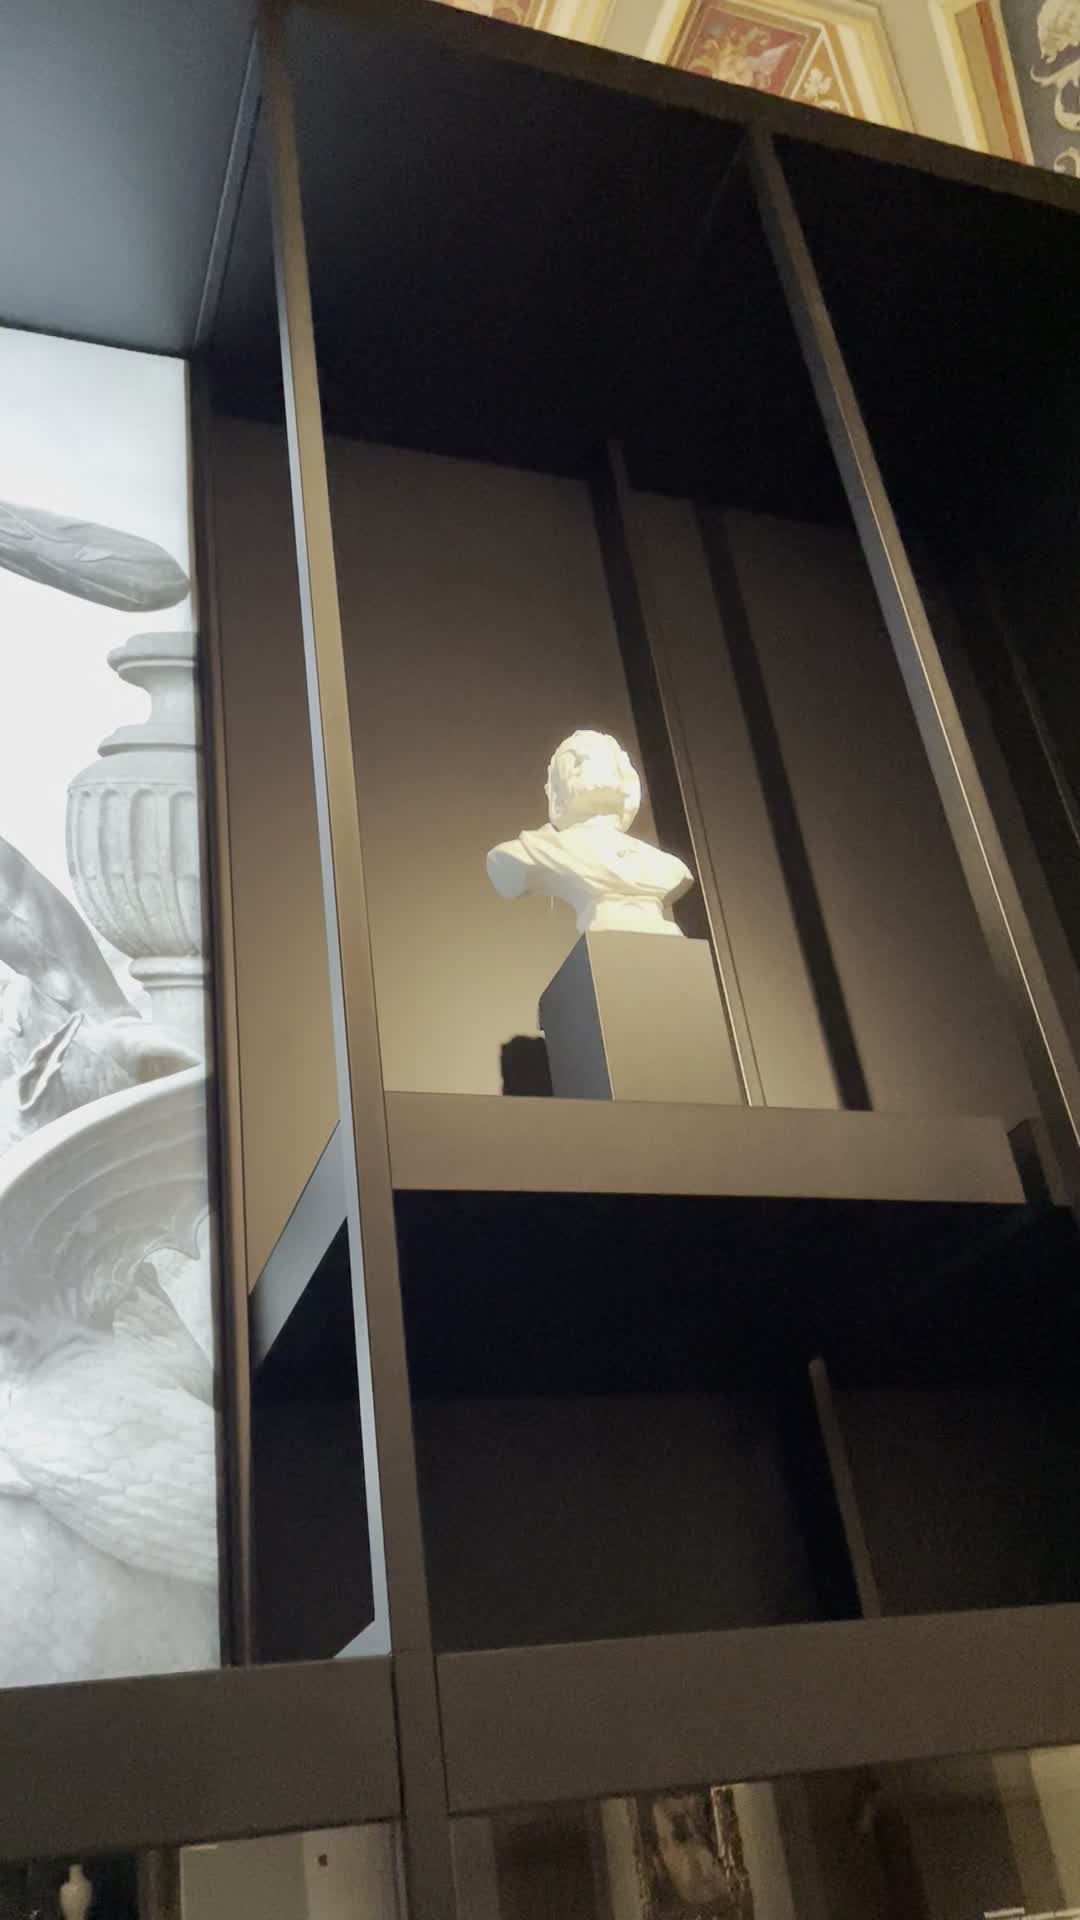
\includegraphics[width=\textwidth]{img/87.jpg}
        \caption{Image of the predicted label 87.}
    \end{subfigure}

    \caption{Misclassified images with their true labels and model predictions (1/2).}\label{fig:misclassifications_examples1}
\end{figure}

\begin{figure}[h]
    \centering

    \begin{subfigure}[b]{0.4\textwidth}
        \centering
        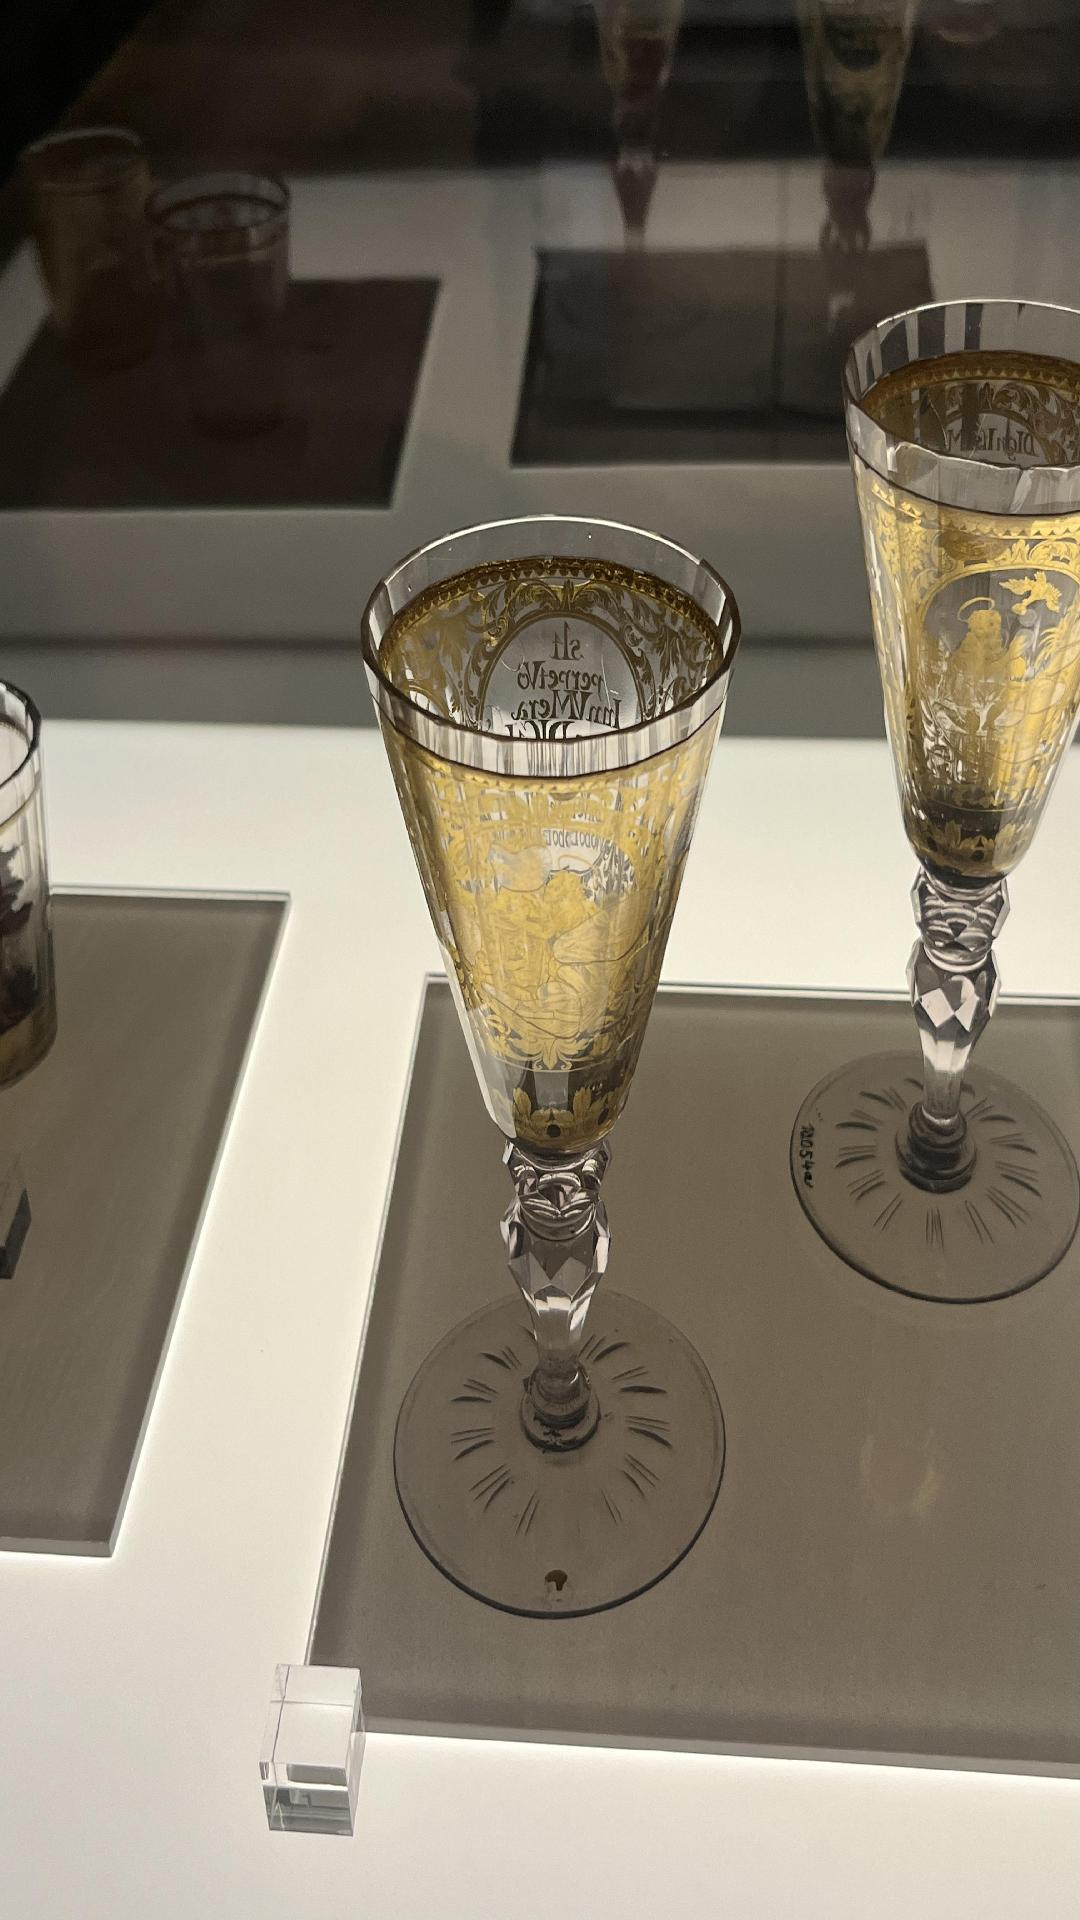
\includegraphics[width=\textwidth]{img/117.jpg}
        \caption{Input image with true label 117.}
    \end{subfigure}
    \hfill
    \begin{subfigure}[b]{0.4\textwidth}
        \centering
        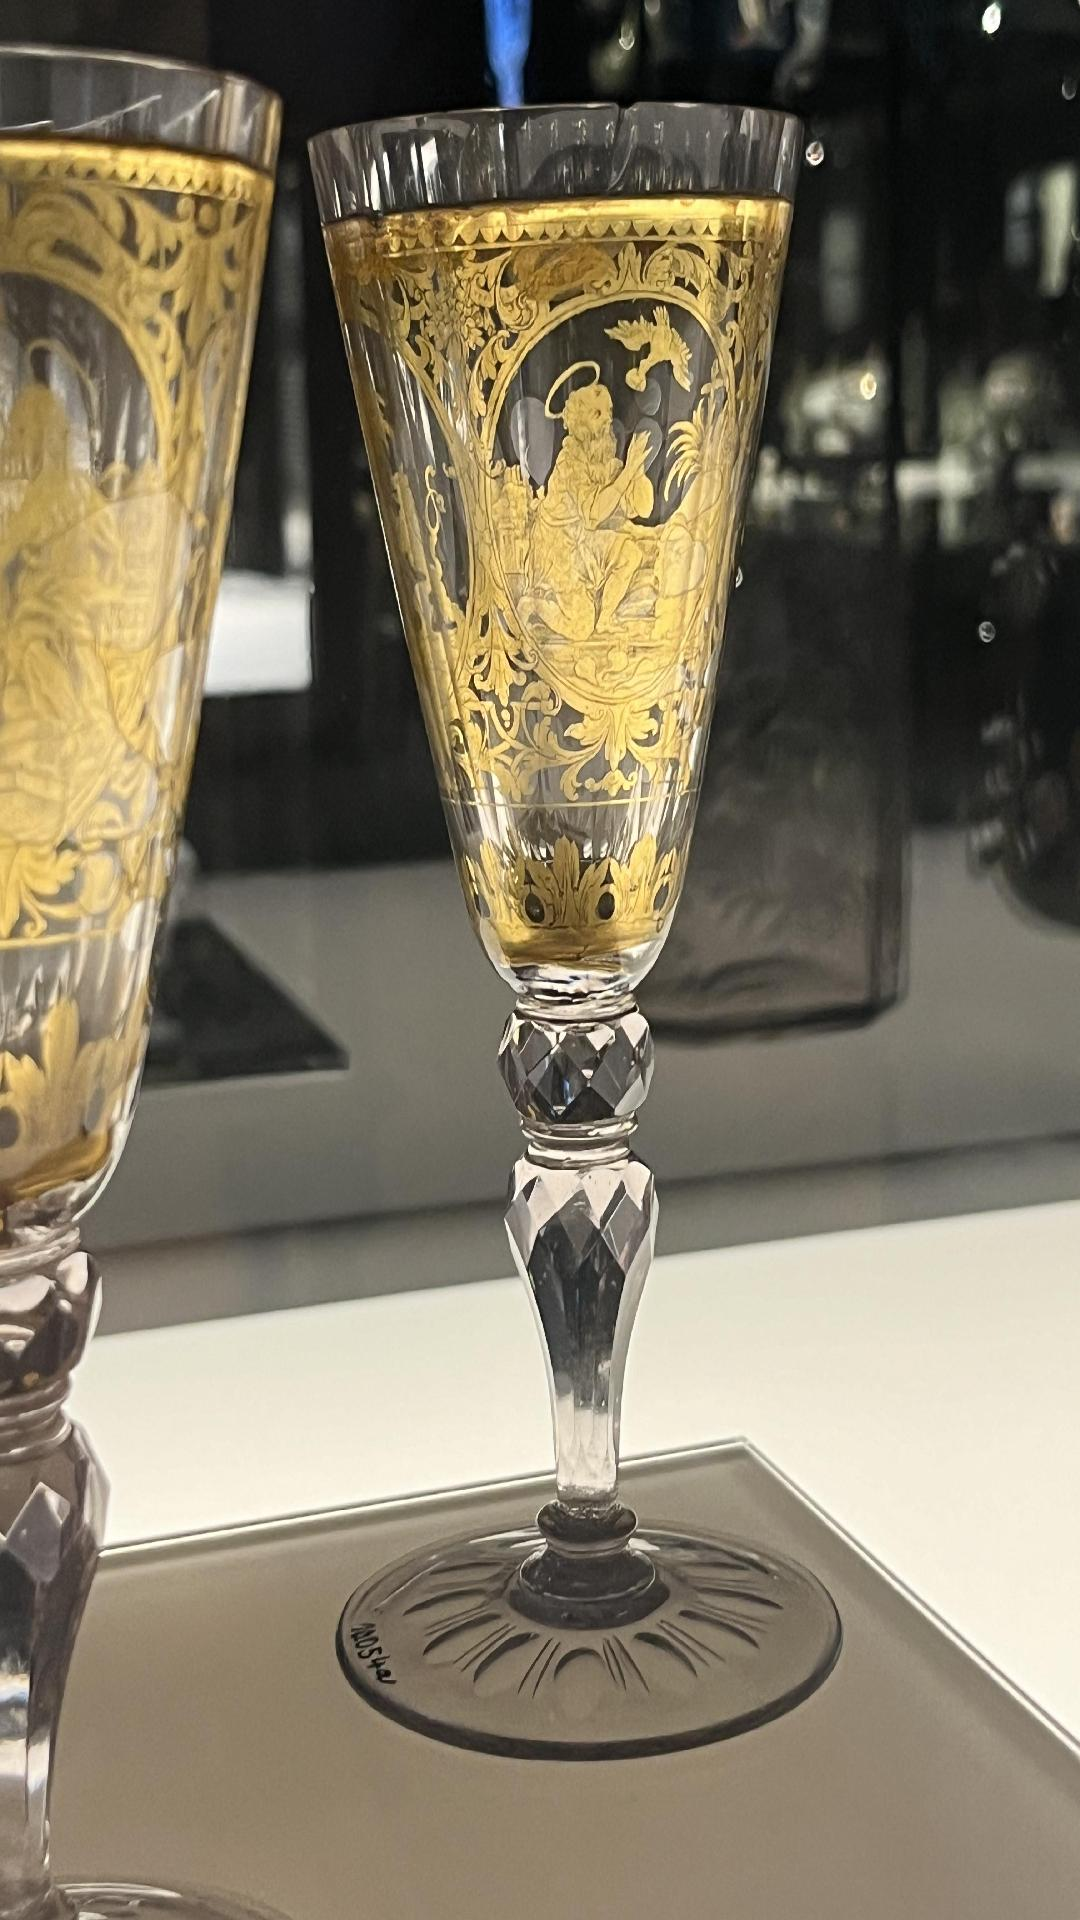
\includegraphics[width=\textwidth]{img/118.jpg}
        \caption{Image of the predicted label 118.}
    \end{subfigure}

    \vspace{1em}

    \begin{subfigure}[b]{0.4\textwidth}
        \centering
        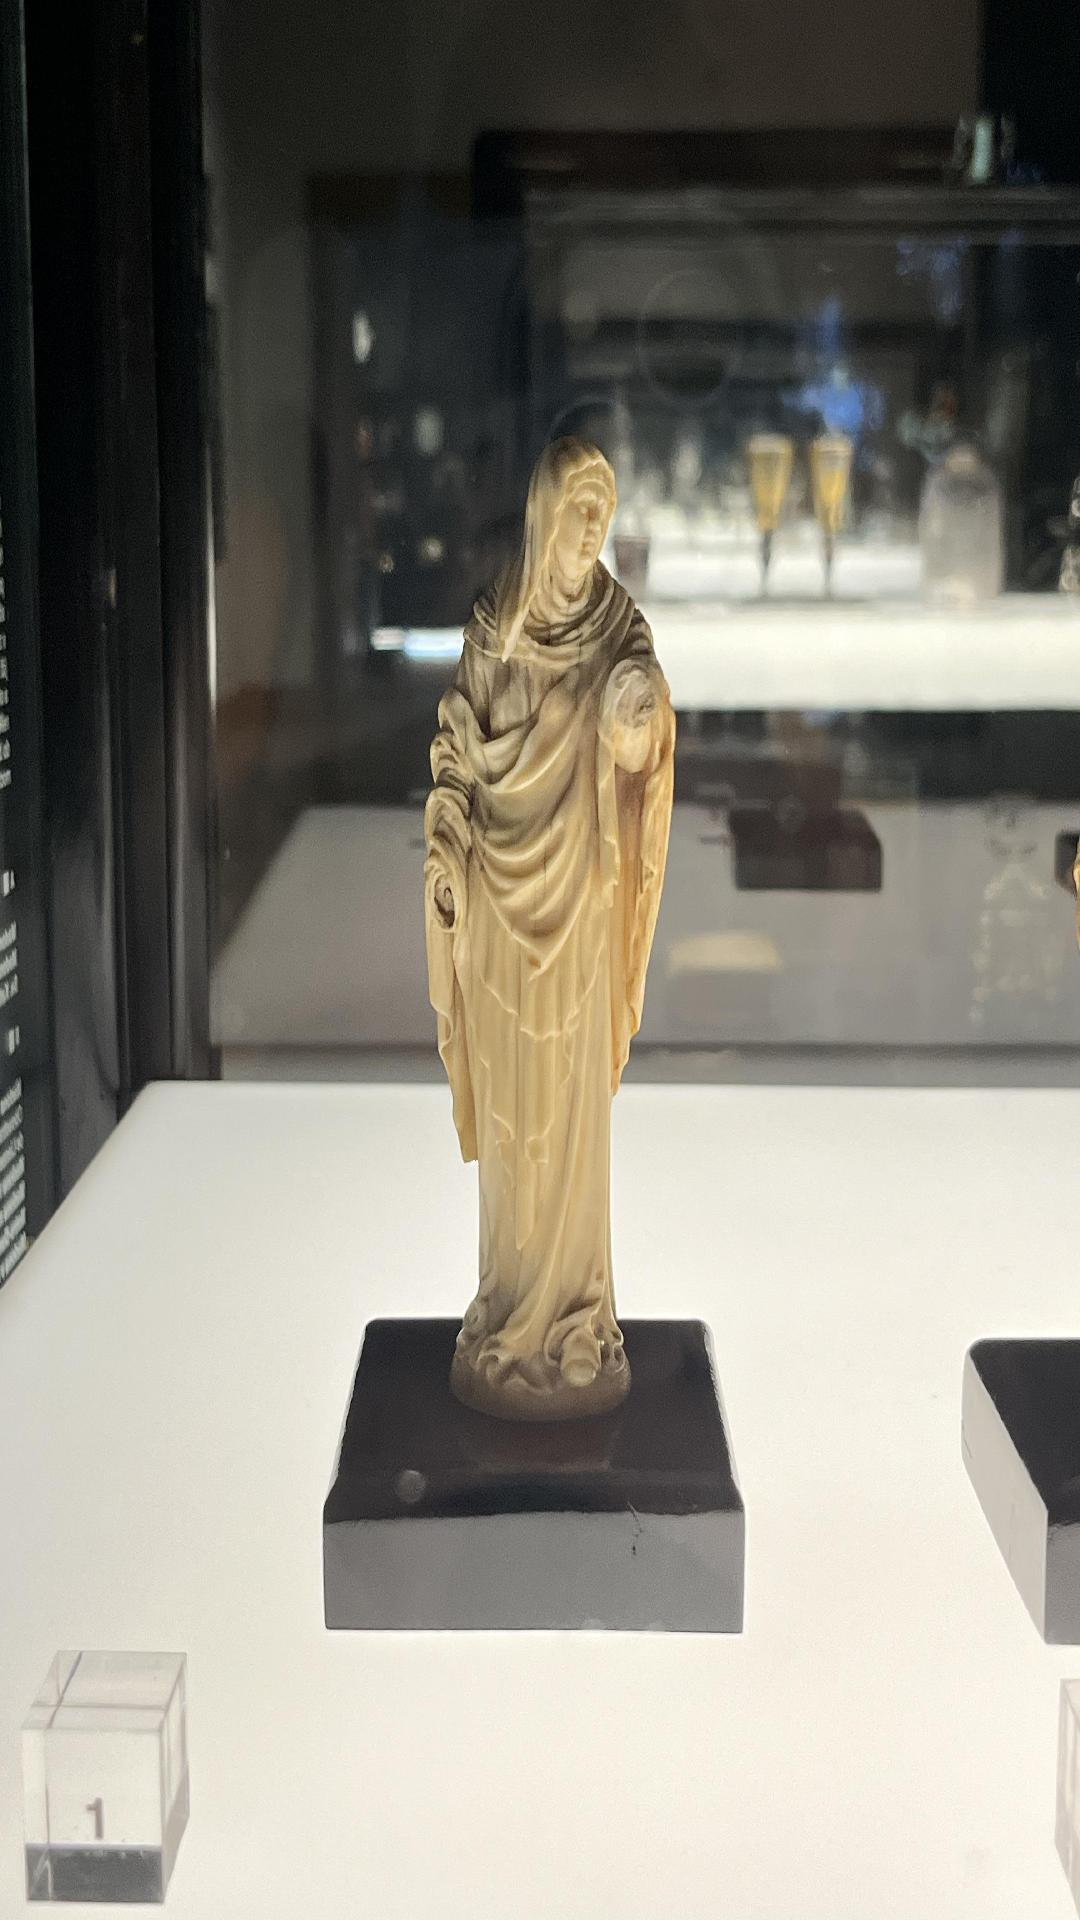
\includegraphics[width=\textwidth]{img/110.jpg}
        \caption{Input image with true label 110.}
    \end{subfigure}
    \hfill
    \begin{subfigure}[b]{0.4\textwidth}
        \centering
        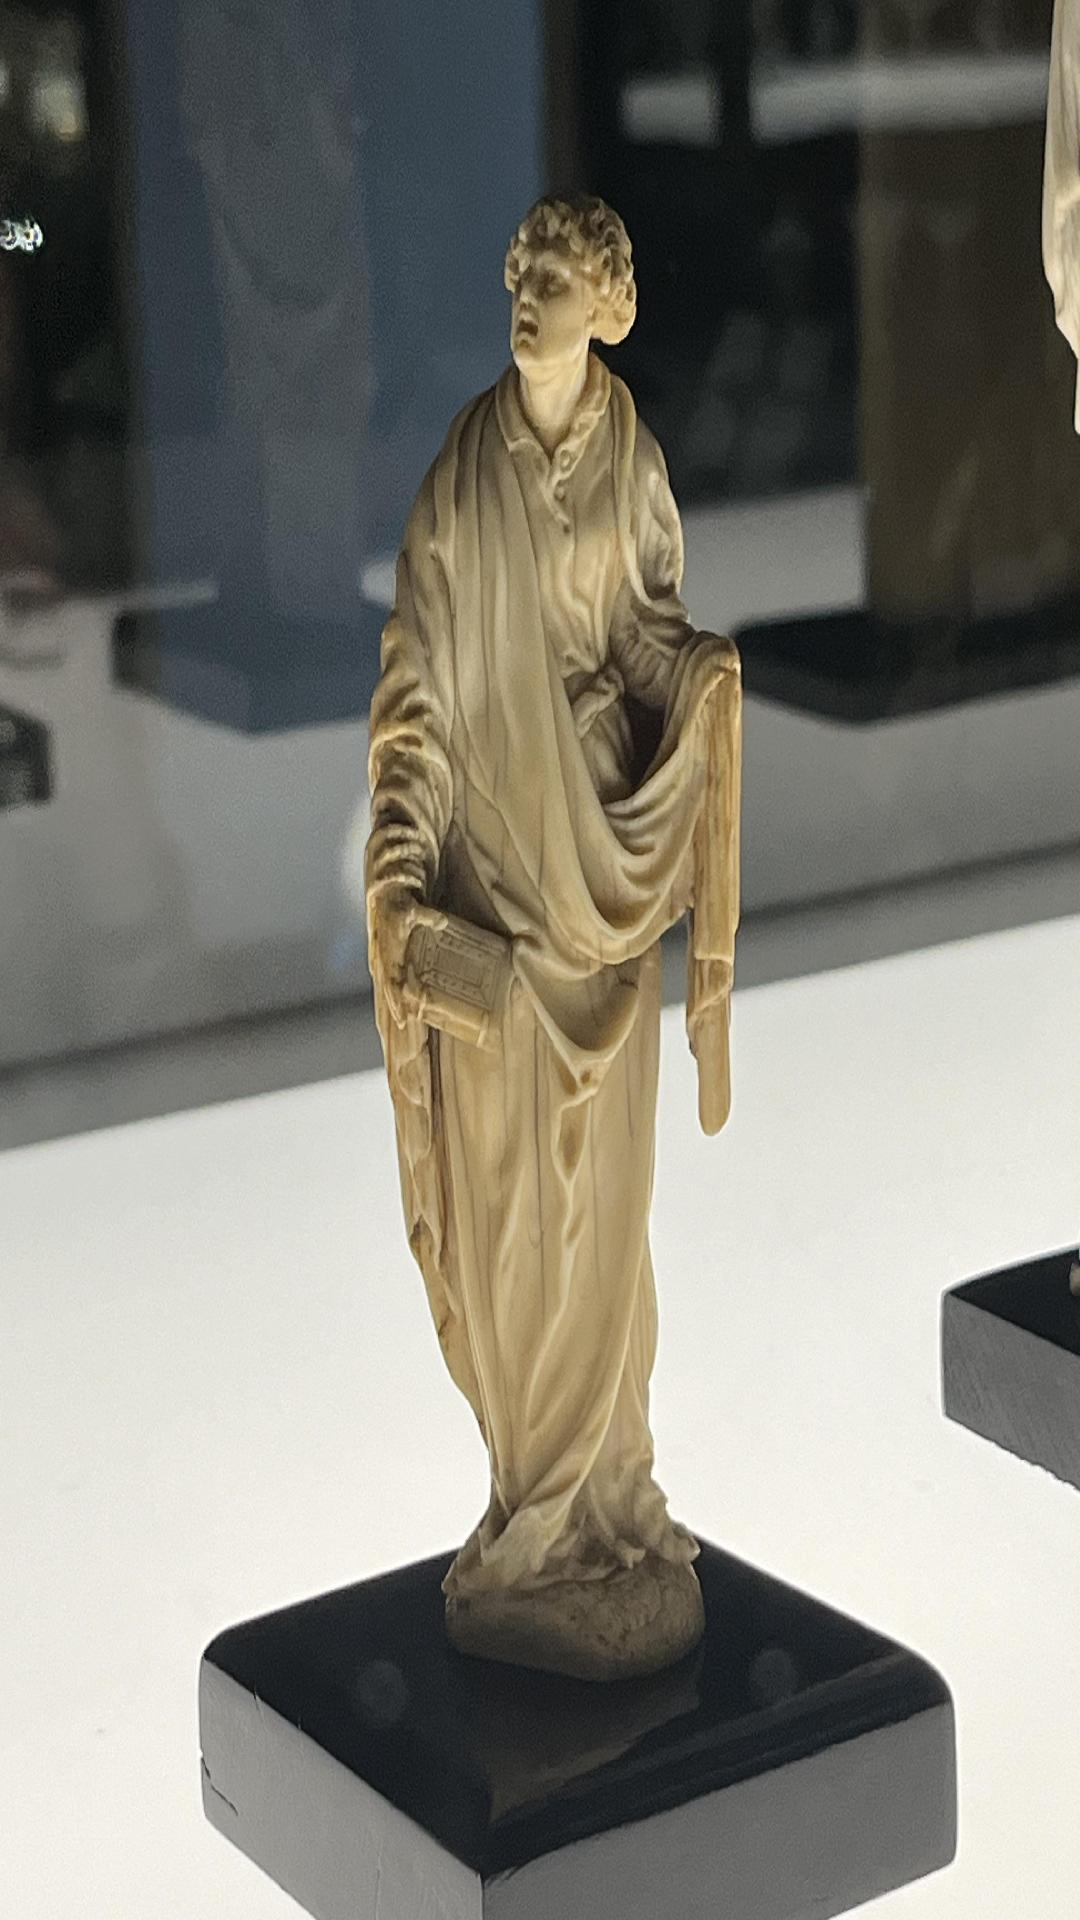
\includegraphics[width=\textwidth]{img/111.jpg}
        \caption{Image of the predicted label 111.}
    \end{subfigure}

    \caption{Misclassified images with their true labels and model predictions (2/2).}\label{fig:misclassifications_examples2}
\end{figure}


\section{TensorFlow Lite}

The trained model was converted to TensorFlow Lite format to use the model on mobile devices. TensorFlow Lite (now known as LiteRT~\cite{tensorflow_lite}) reduces model size and complexity, allowing it to run quickly on smartphones. The conversion was done using TensorFlow's built-in converter (TFLiteConverter), compressing the model without losing much accuracy.

\section{Conclusion}

In this chapter, we have described the process of training a machine learning model to recognize museum exhibits. We explored different approaches, ultimately selecting transfer learning with the MobileNetV2 architecture. The model was trained on a dataset of frames extracted from video recordings of exhibits, achieving a validation accuracy of 0.959 after fine-tuning.

We also analyzed the misclassifications made by the model, identifying patterns in errors and providing insights into addressing these errors. The model was converted to TensorFlow Lite format for deployment on mobile devices, ensuring efficient performance in real-time exhibit recognition.
\chapter{Android Application Development}

\section{Choice of Platform}

We chose Android as the target platform because it remains the most popular mobile operating system globally, holding approximately 70\% of the market share as of 2025. While cross-platform solutions like React Native, Flutter, or Xamarin offer the advantage of developing for multiple platforms simultaneously, they often come with trade-offs, such as reduced access to native device features, performance overhead, or difficulties integrating specific hardware functionalities. Given our application's requirements for real-time image processing and machine learning integration, native Android development provided the necessary performance and access to device-specific capabilities.

\section{Application Architecture}

The Android application was developed using Kotlin and structured as follows:

\begin{itemize}
\item \textbf{UI}: Contains theming elements such as color schemes, typography, and theme configurations using Jetpack Compose (a modern toolkit for building native UI in Android~\cite{jetpack_compose}). This simplifies the management of visual consistency throughout the app.
\item \textbf{Domain}: Includes core logic and data structures, such as the Classification data class, the IClassifier interface, and image processing helpers. Additionally, it contains the ImageAnalyzer, which manages the analysis of camera frames for classification.
\item \textbf{Data}: Handles the integration and execution of the TensorFlow Lite model through the TfLiteClassifier class. This includes loading the model, preparing images for inference, and providing classification results to the domain layer.
\item \textbf{Root}: Comprises main components directly tied to the application's functionality, such as screens (Home, Gallery, ExhibitDetailScreen, PhotoScanner) and navigation between these screens.
\end{itemize}

This organization separates responsibilities, keeping the project maintainable.

\section{User Interface}

There are five main screens in the application:

\begin{itemize}
\item \textbf{Home Screen}: A page dedicated to the museum, with contacts and social media links.
\item \textbf{Gallery Screen}: A page displaying a grid of museum exhibits, allowing users to browse through available items and open detailed information about each exhibit.
\item \textbf{Exhibit Detail Screen}: A page providing information about an exhibit, such as title, author, and dates.
\item \textbf{Photo Scanner Screen}: Presents real-time recognition results directly overlaid on the live camera view.
\item \textbf{Classification Result Screen}: Displays the classification results, showing the top recognized exhibit and up to four alternatives for user selection ordered by confidence level. This is particularly useful for misclassified or uncertain results, allowing users to find the correct exhibit.
\end{itemize}

TODO: Add screenshots of the application

\section{Real-Time Image Processing and TensorFlow Lite Integration}

To make our application recognize museum exhibits in real-time, we combined the capabilities of TensorFlow Lite (TFLite) with Android's CameraX library~\cite{camerax}. TensorFlow Lite allows machine learning models to run efficiently directly on mobile devices, while CameraX makes it straightforward to access and manage the device's camera hardware across various Android phones.

When the application starts, it loads the MobileNetV2 TFLite model we trained. This initial loading is done once.

Next, CameraX continuously captures frames from the camera. To avoid overwhelming the device, our application analyzes only every 30th frame captured by the camera. This balance provides timely recognition without putting too much strain on the phone's resources.

Each captured frame is initially in YUV format, a standard camera format optimized for speed and efficiency. However, our model requires standard Bitmap images, representing image data in the RGB color space. Therefore, each selected YUV frame is converted into a Bitmap.

After converting to a Bitmap, we preprocess the image further by resizing it to $224 \times 224$ pixels to match the input dimensions of the MobileNetV2 model. Additionally, each pixel's values are normalized, adjusting them from the original 0--255 range into a 0--1 range. This normalization is crucial for the model to interpret the pixel values correctly, as it was trained on images in this normalized format.

Once preprocessed, the Bitmap is sent to the TensorFlow Lite model, which performs the classification task. The model analyzes the image and returns a set of predictions, ranking them based on confidence levels. These results are then sent to the UI, where users can see the recognized exhibit and alternative suggestions to help with possible misclassifications.

By integrating CameraX for capturing frames and TensorFlow Lite for image recognition, we created an efficient, responsive application that provides museum visitors with immediate and reliable exhibit identification.

\section{Conclusion}

In this chapter, we have described in detail the development of our Android application, focusing on the choice of platform, architecture, user interface design, and integration of real-time image processing with TensorFlow Lite. The application is designed in such a way as to ensure user-friendliness while efficiently using the device's resources to recognize exhibits in real time. The combination of CameraX and TensorFlow Lite allows you to effectively classify museum exhibits, increasing visitor engagement and interaction with the museum's offerings.
\chapter{Results}

This chapter presents the outcomes of testing the developed mobile application for real-time museum exhibit recognition. The evaluation was conducted directly at the Museum of Decorative Arts in Prague (\textit{Uměleckoprůmyslové museum v Praze} or UPM), where the videos for our training dataset were recorded. UPM gathers, curates, and preserves historical and contemporary collections of applied arts, design, and artistic craftsmanship for future generations. The main goal for this testing was to verify whether the performance achieved in the initial validation phase (Chapter~\ref{chapter:model_training}) corresponds with real-world application scenarios within the museum environment.

\section{Testing Procedure}

The guidelines were established before testing to maintain consistency and repeatability. Each test was performed by pointing the smartphone camera at selected museum exhibits from different but reasonable angles, trying to replicate typical user scenarios. The testing was conducted twice: in the morning and in the evening, allowing us to measure the model's robustness under different lighting conditions (which, however, were not much different due to the museum's indoor lighting). The application was run on a Samsung Galaxy S9 smartphone.

Due to changes in UPM's exhibition collections between the creation of the dataset and the time of testing, not all exhibits initially present in our dataset were still accessible. Therefore, for practical evaluation purposes, we found a subset of 80 available exhibits covering a diverse range of kinds and sizes, including furniture, sculptures, paintings, clothes, toys, jewelry, and glass art.

\section{Classification Results and Accuracy}

The results were the same for both morning and evening testing. Out of the 80 exhibits chosen for the evaluation, the application correctly identified 75 of them at the first attempt, which equals an accuracy rate of approximately 93.75\%. Importantly, the five misclassified exhibits were nevertheless found among the alternative predictions displayed to the user.

Three of the five misclassifications were sculptures, which were visually similar to one another, and the remaining two were a glass artwork and a painting, which again had very similar counterparts in the training dataset. The model was the most confident about toys and furniture, since there was much more diversity between them: they were of different shapes, colors, and sizes, while the sculptures were more challenging due to their similar forms and materials.

This result aligns closely with our validation set results obtained during the training phase (where validation accuracy was around 95.9\% after fine-tuning). Observing that real-world accuracy was only slightly lower is encouraging, as this confirms that the model is generalizing appropriately.

\section{Inference Time and Responsiveness}

A critical aspect of our testing was checking the application's real-time responsiveness, as slow predictions would negatively affect user experience. Thanks to the implemented Debug Mode, inference time measurements (the time required for the model to produce predictions from input images) could be observed and recorded directly within the mobile application during testing.

On average, inference times remained stable at around 120--150 ms. This performance is beneficial for seamless and smooth recognition, especially important when visitors move with their devices through exhibitions. Such fast classification guarantees minimal latency observable to the human eye, providing an actual real-time experience. Additionally, the achieved inference time would not have been possible with alternative methods such as the embedding-based similarity search approach, which typically requires more extensive search space computations. Thus, our chosen method, direct classification via MobileNetV2 and TensorFlow Lite integration, was confirmed to be the most suitable for practical museum deployments on mobile devices.

\section{Confidence Levels and Threshold Evaluation}

During the real-world testing sessions, we also monitored prediction confidence levels generated by the model to assess our chosen classification threshold value (0.3). For most correctly identified exhibits, the confidence scores ranged between 0.5 and 1.0. Typically, larger and visually distinguishable items were consistently predicted with confidence values above 0.8, whereas smaller or visually less distinctive exhibits fell towards lower confidence scores, around 0.5--0.7.

Nevertheless, despite observing relatively higher confidence values for correctly classified items, we maintained the lower threshold of 0.3 initially chosen during development. This was done to ensure that the correct exhibit could still be found among the alternatives even in cases of misclassifications.

\section{Visual Results and Demonstration}

To visually document and illustrate real-world app performance and functioning, several photos and a video were recorded during the evaluation process. In Figure~\ref{fig:test_examples}, you can see some examples of the application recognizing various exhibits in the museum.

\begin{figure}[h]
    \centering

    \begin{subfigure}[b]{0.4\textwidth}
        \centering
        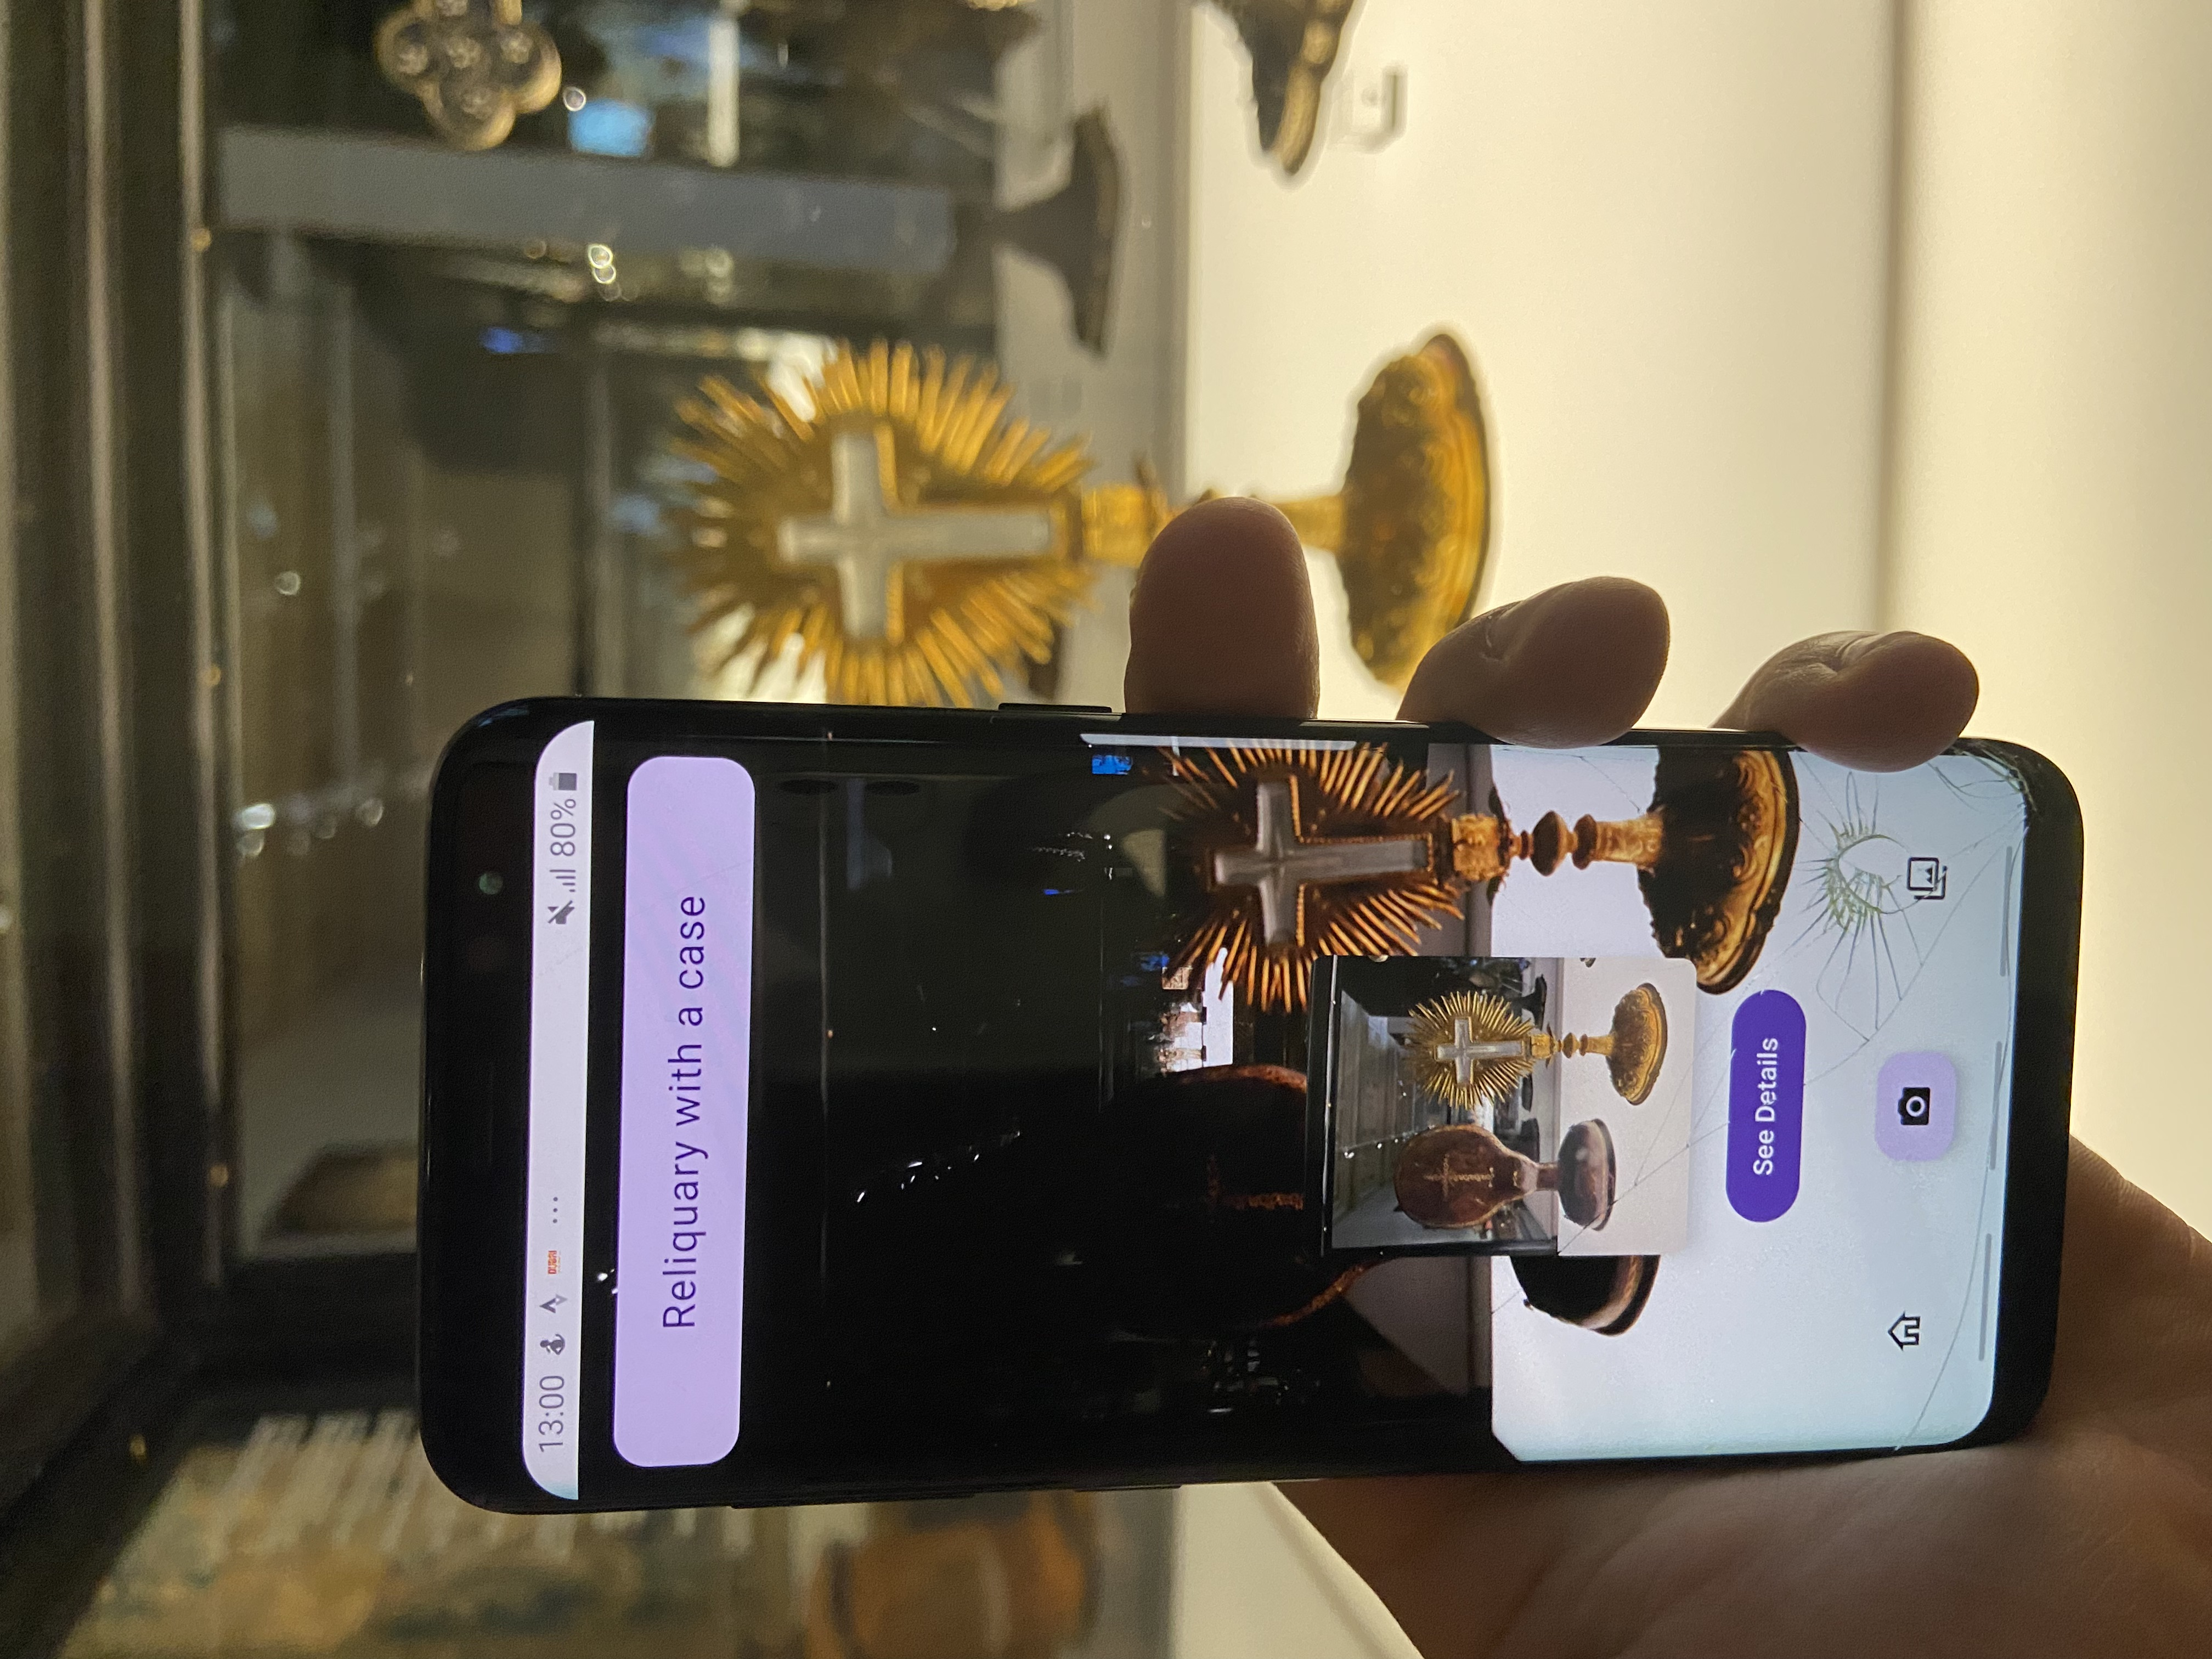
\includegraphics[angle=270, width=\textwidth]{img/test-example-1.jpg}
    \end{subfigure}
    \hfill
    \begin{subfigure}[b]{0.4\textwidth}
        \centering
        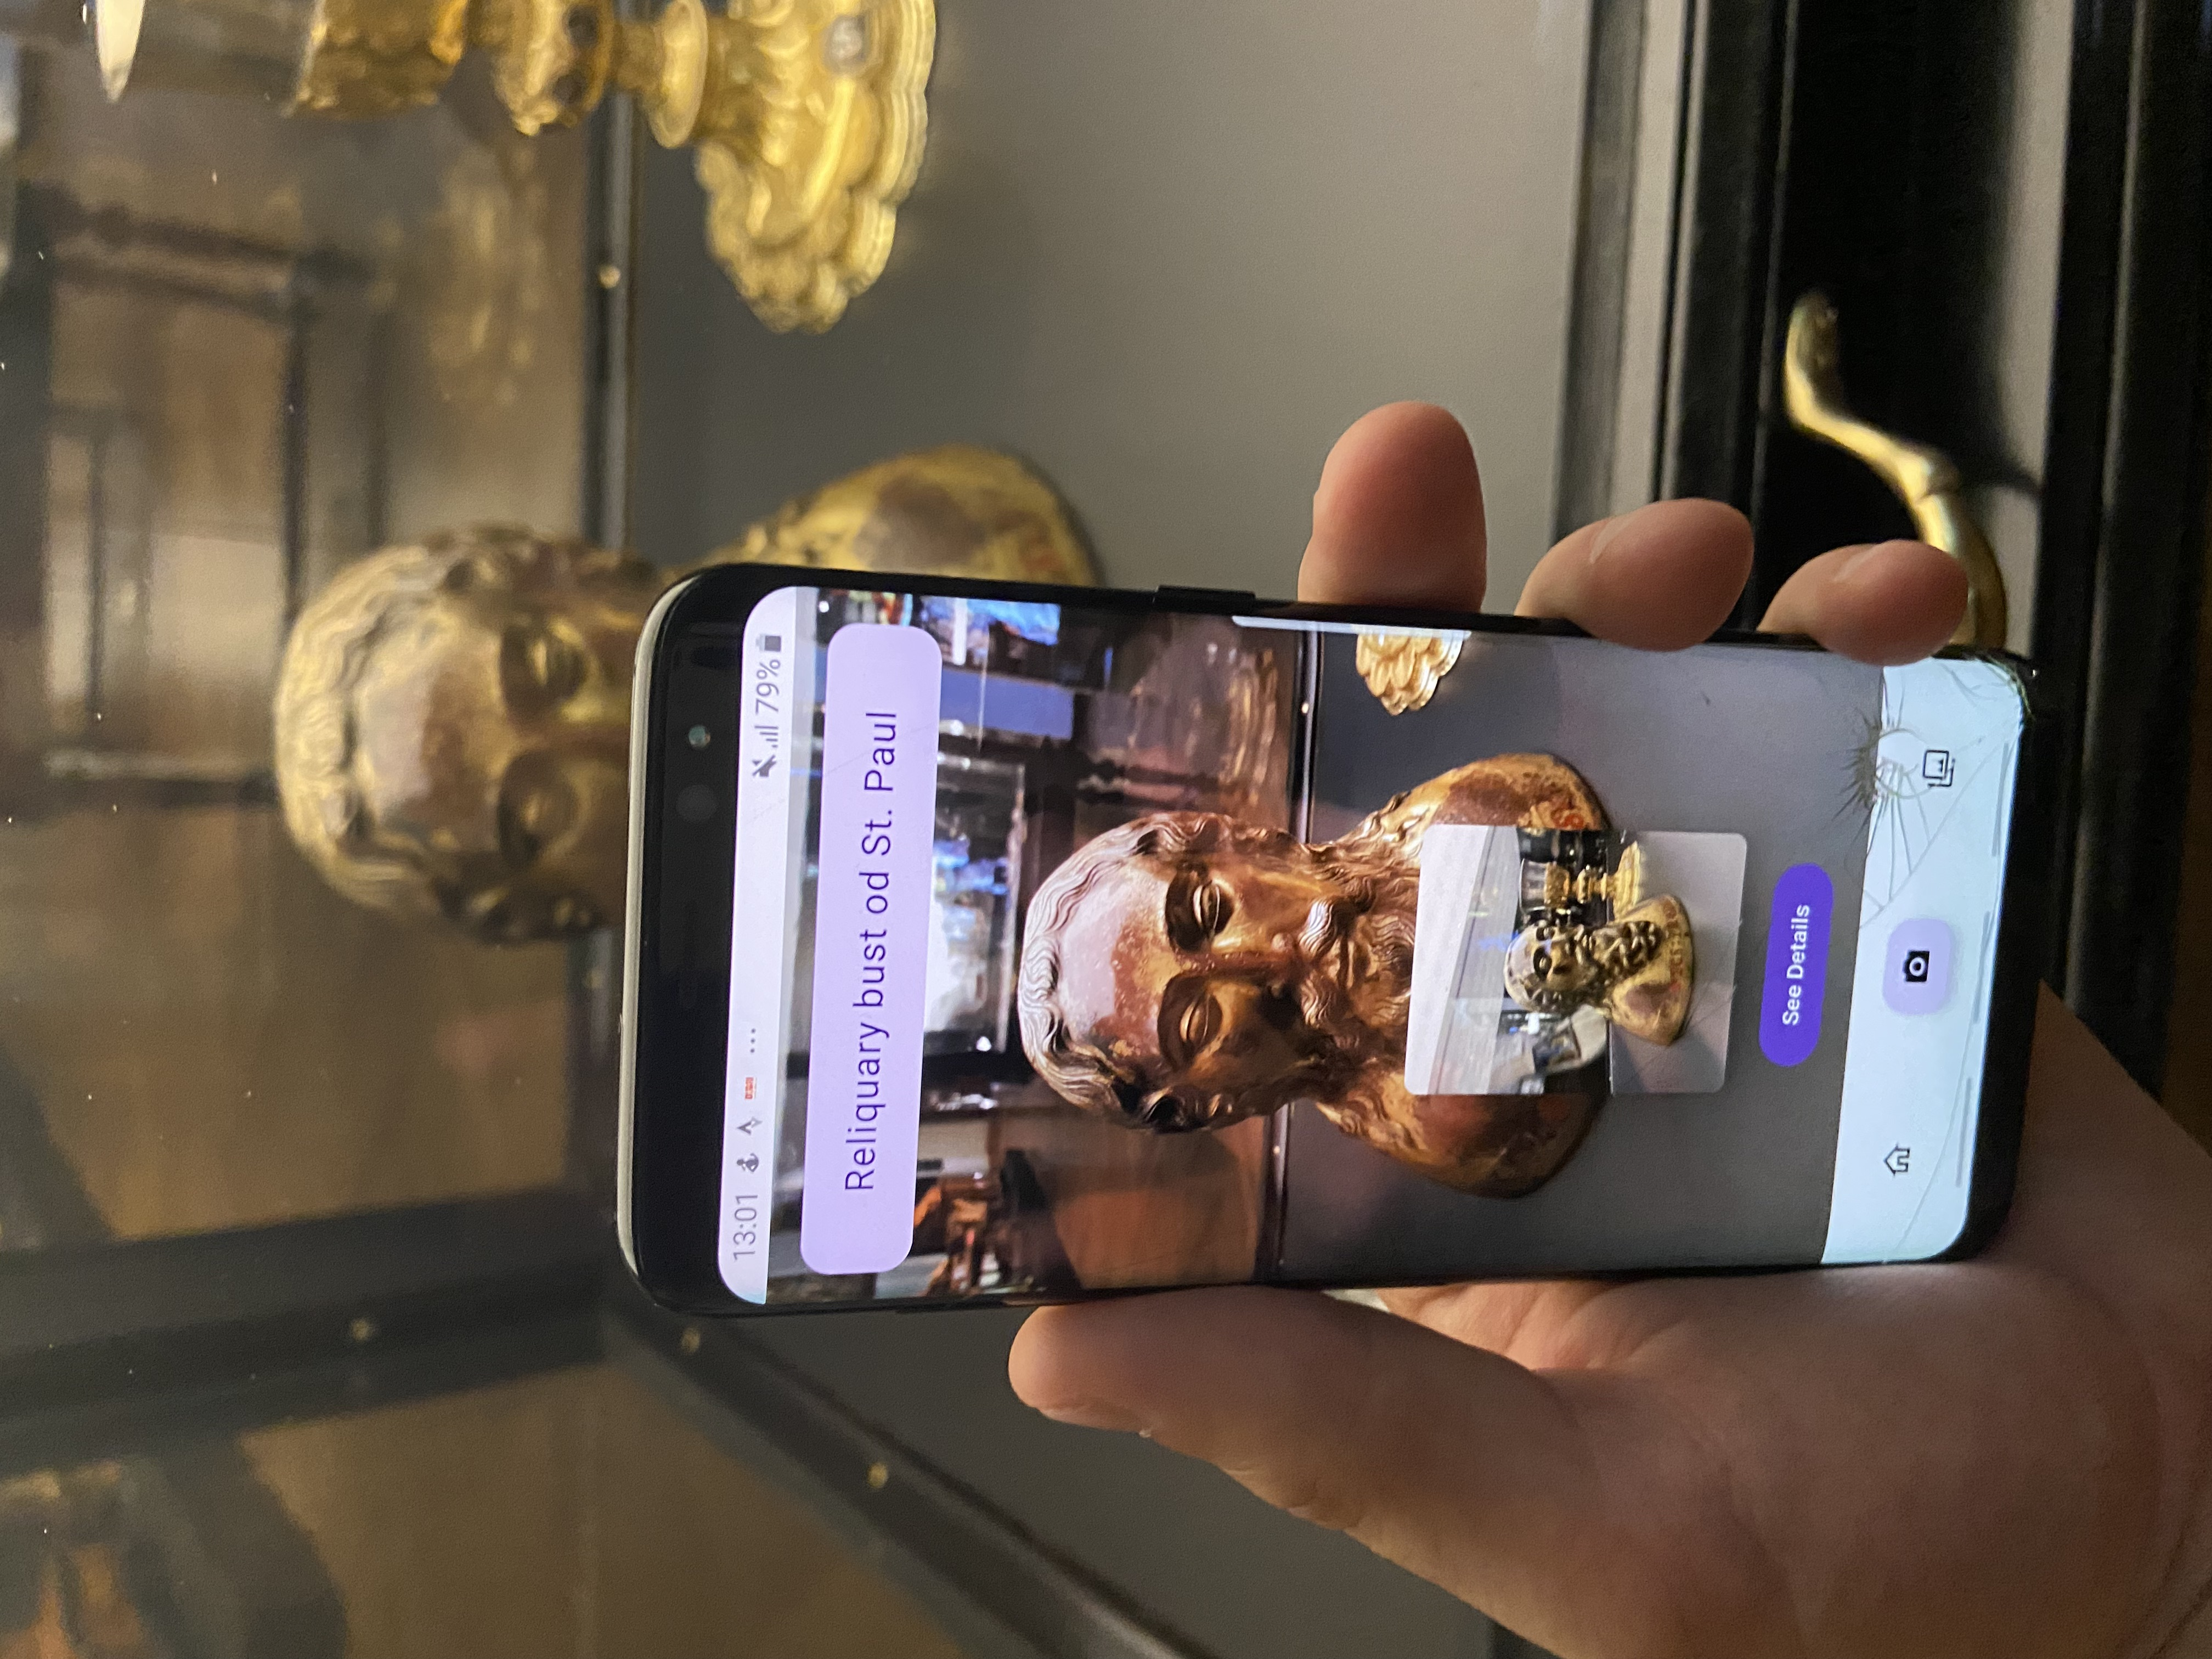
\includegraphics[angle=270, width=\textwidth]{img/test-example-2.jpg}
    \end{subfigure}

    \vspace{1em}

    \begin{subfigure}[b]{0.4\textwidth}
        \centering
        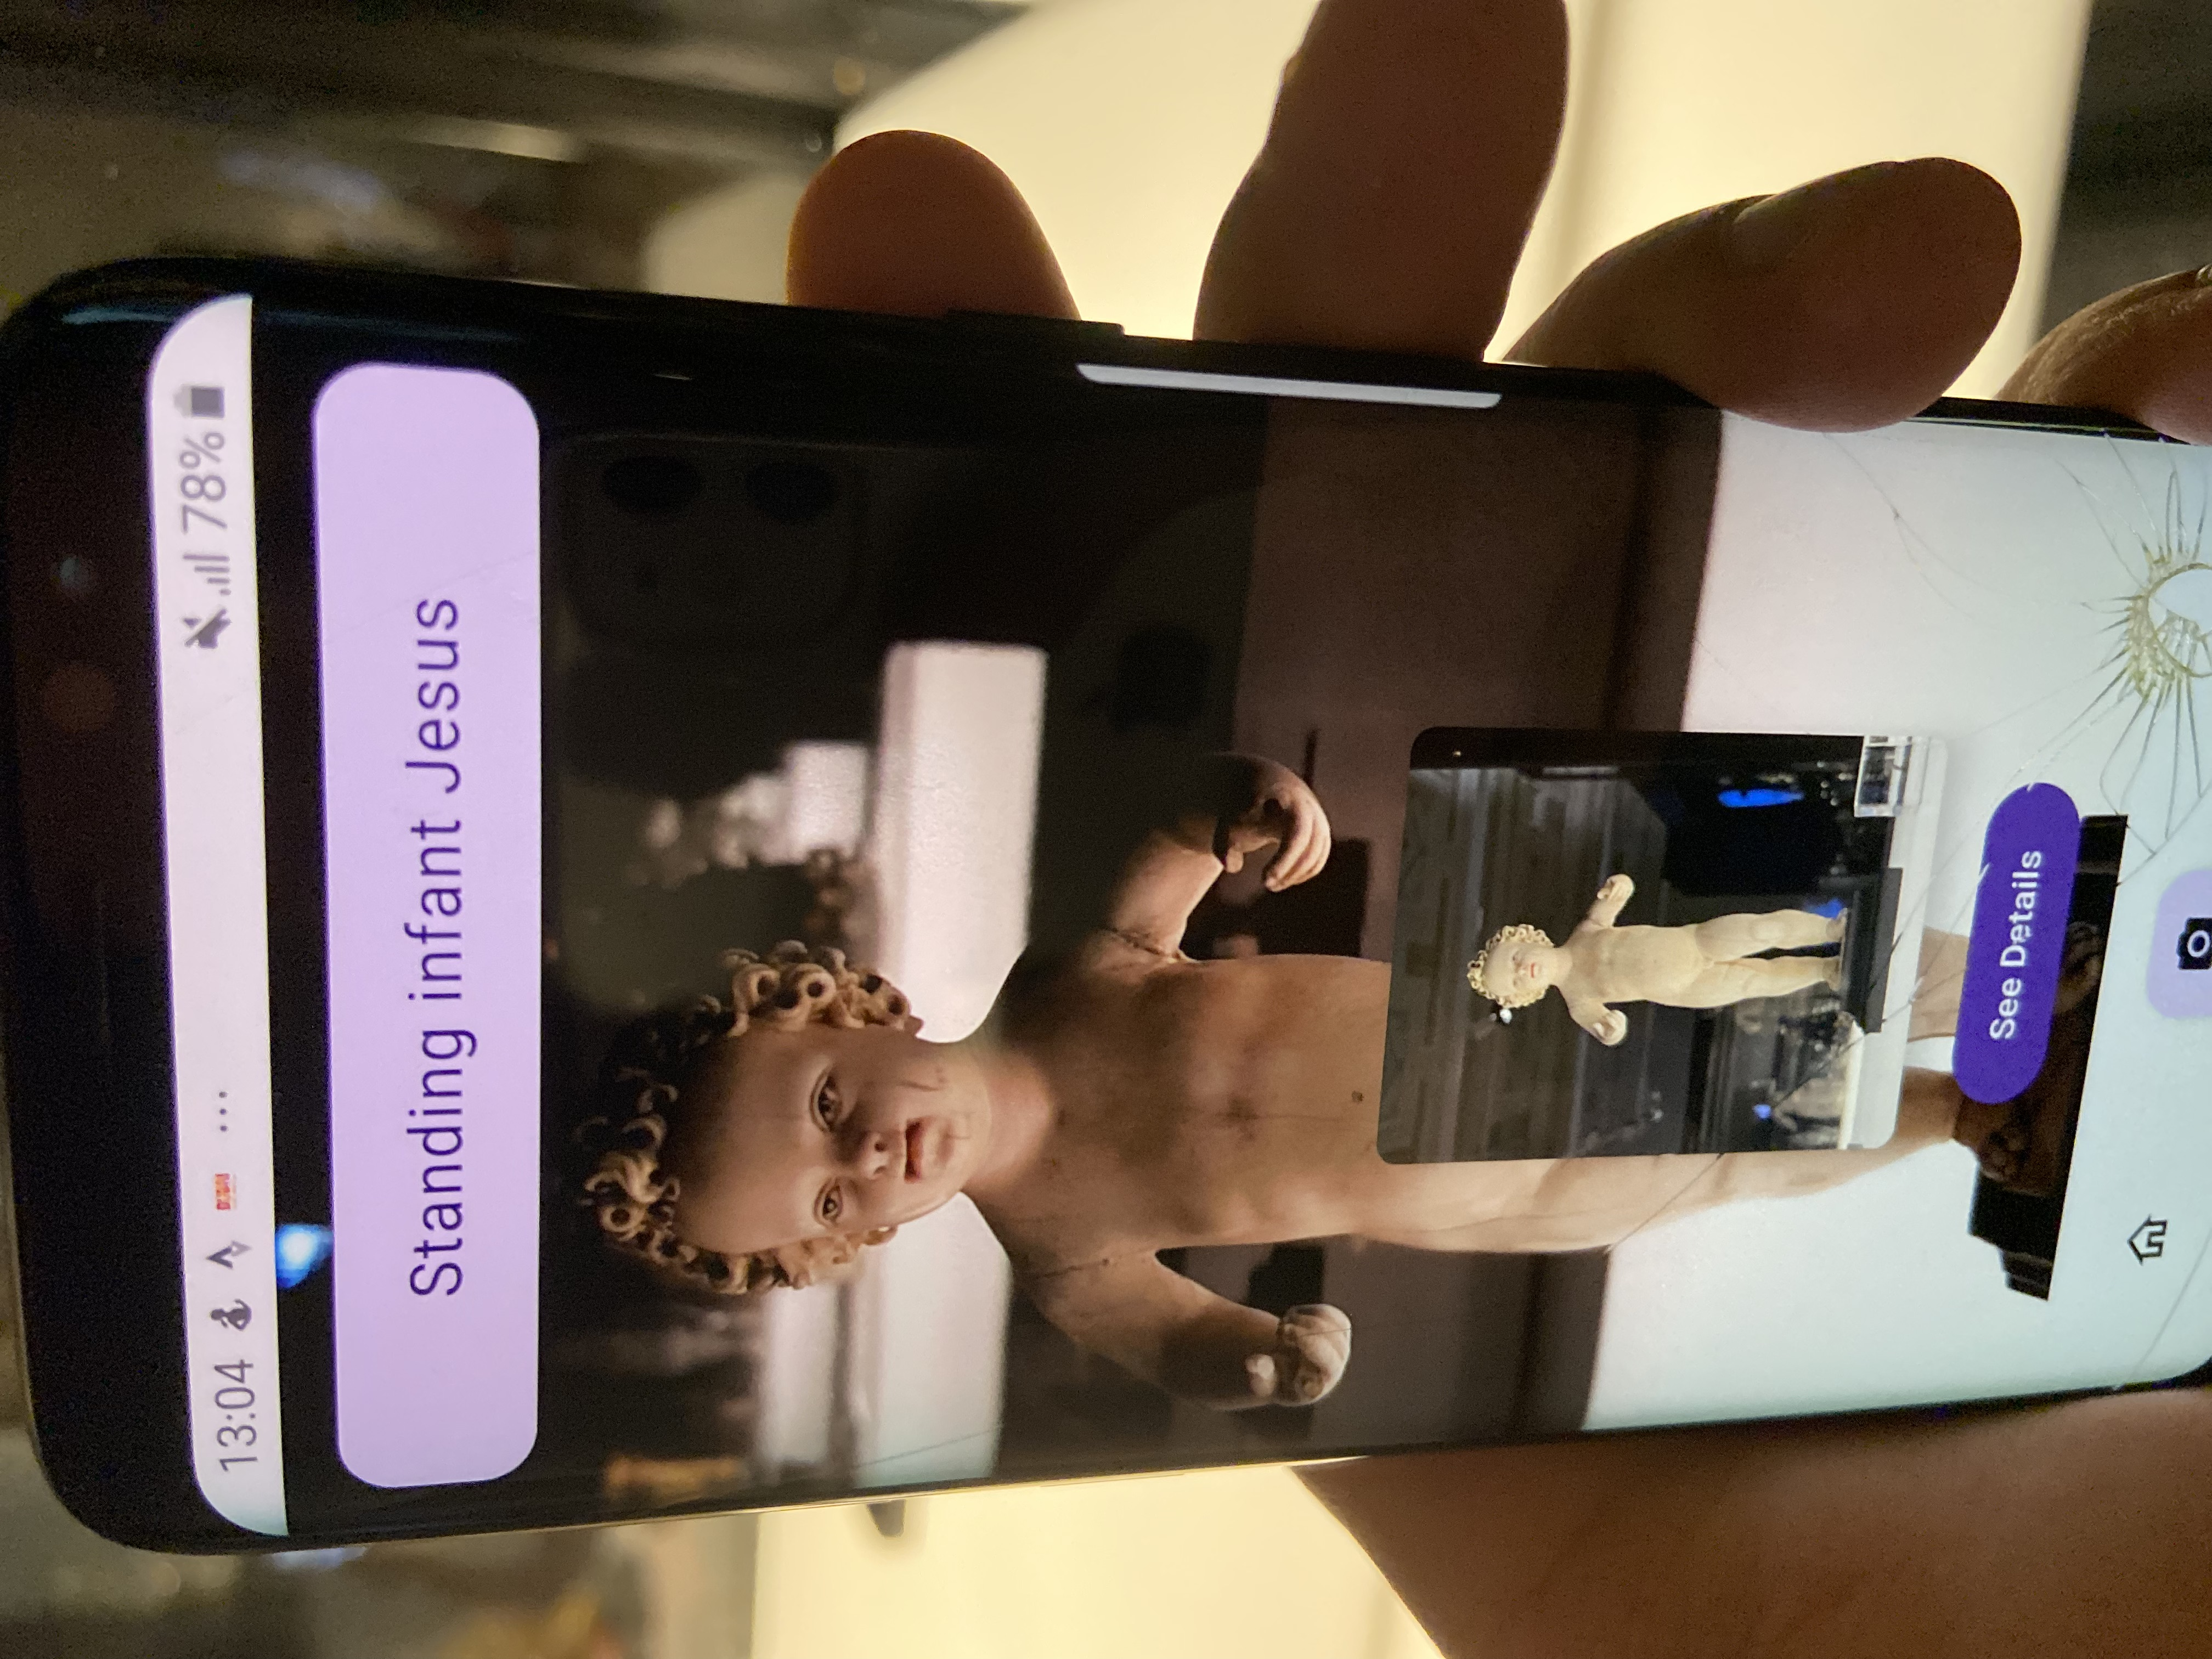
\includegraphics[angle=270, width=\textwidth]{img/test-example-3.jpg}
    \end{subfigure}
    \hfill
    \begin{subfigure}[b]{0.4\textwidth}
        \centering
        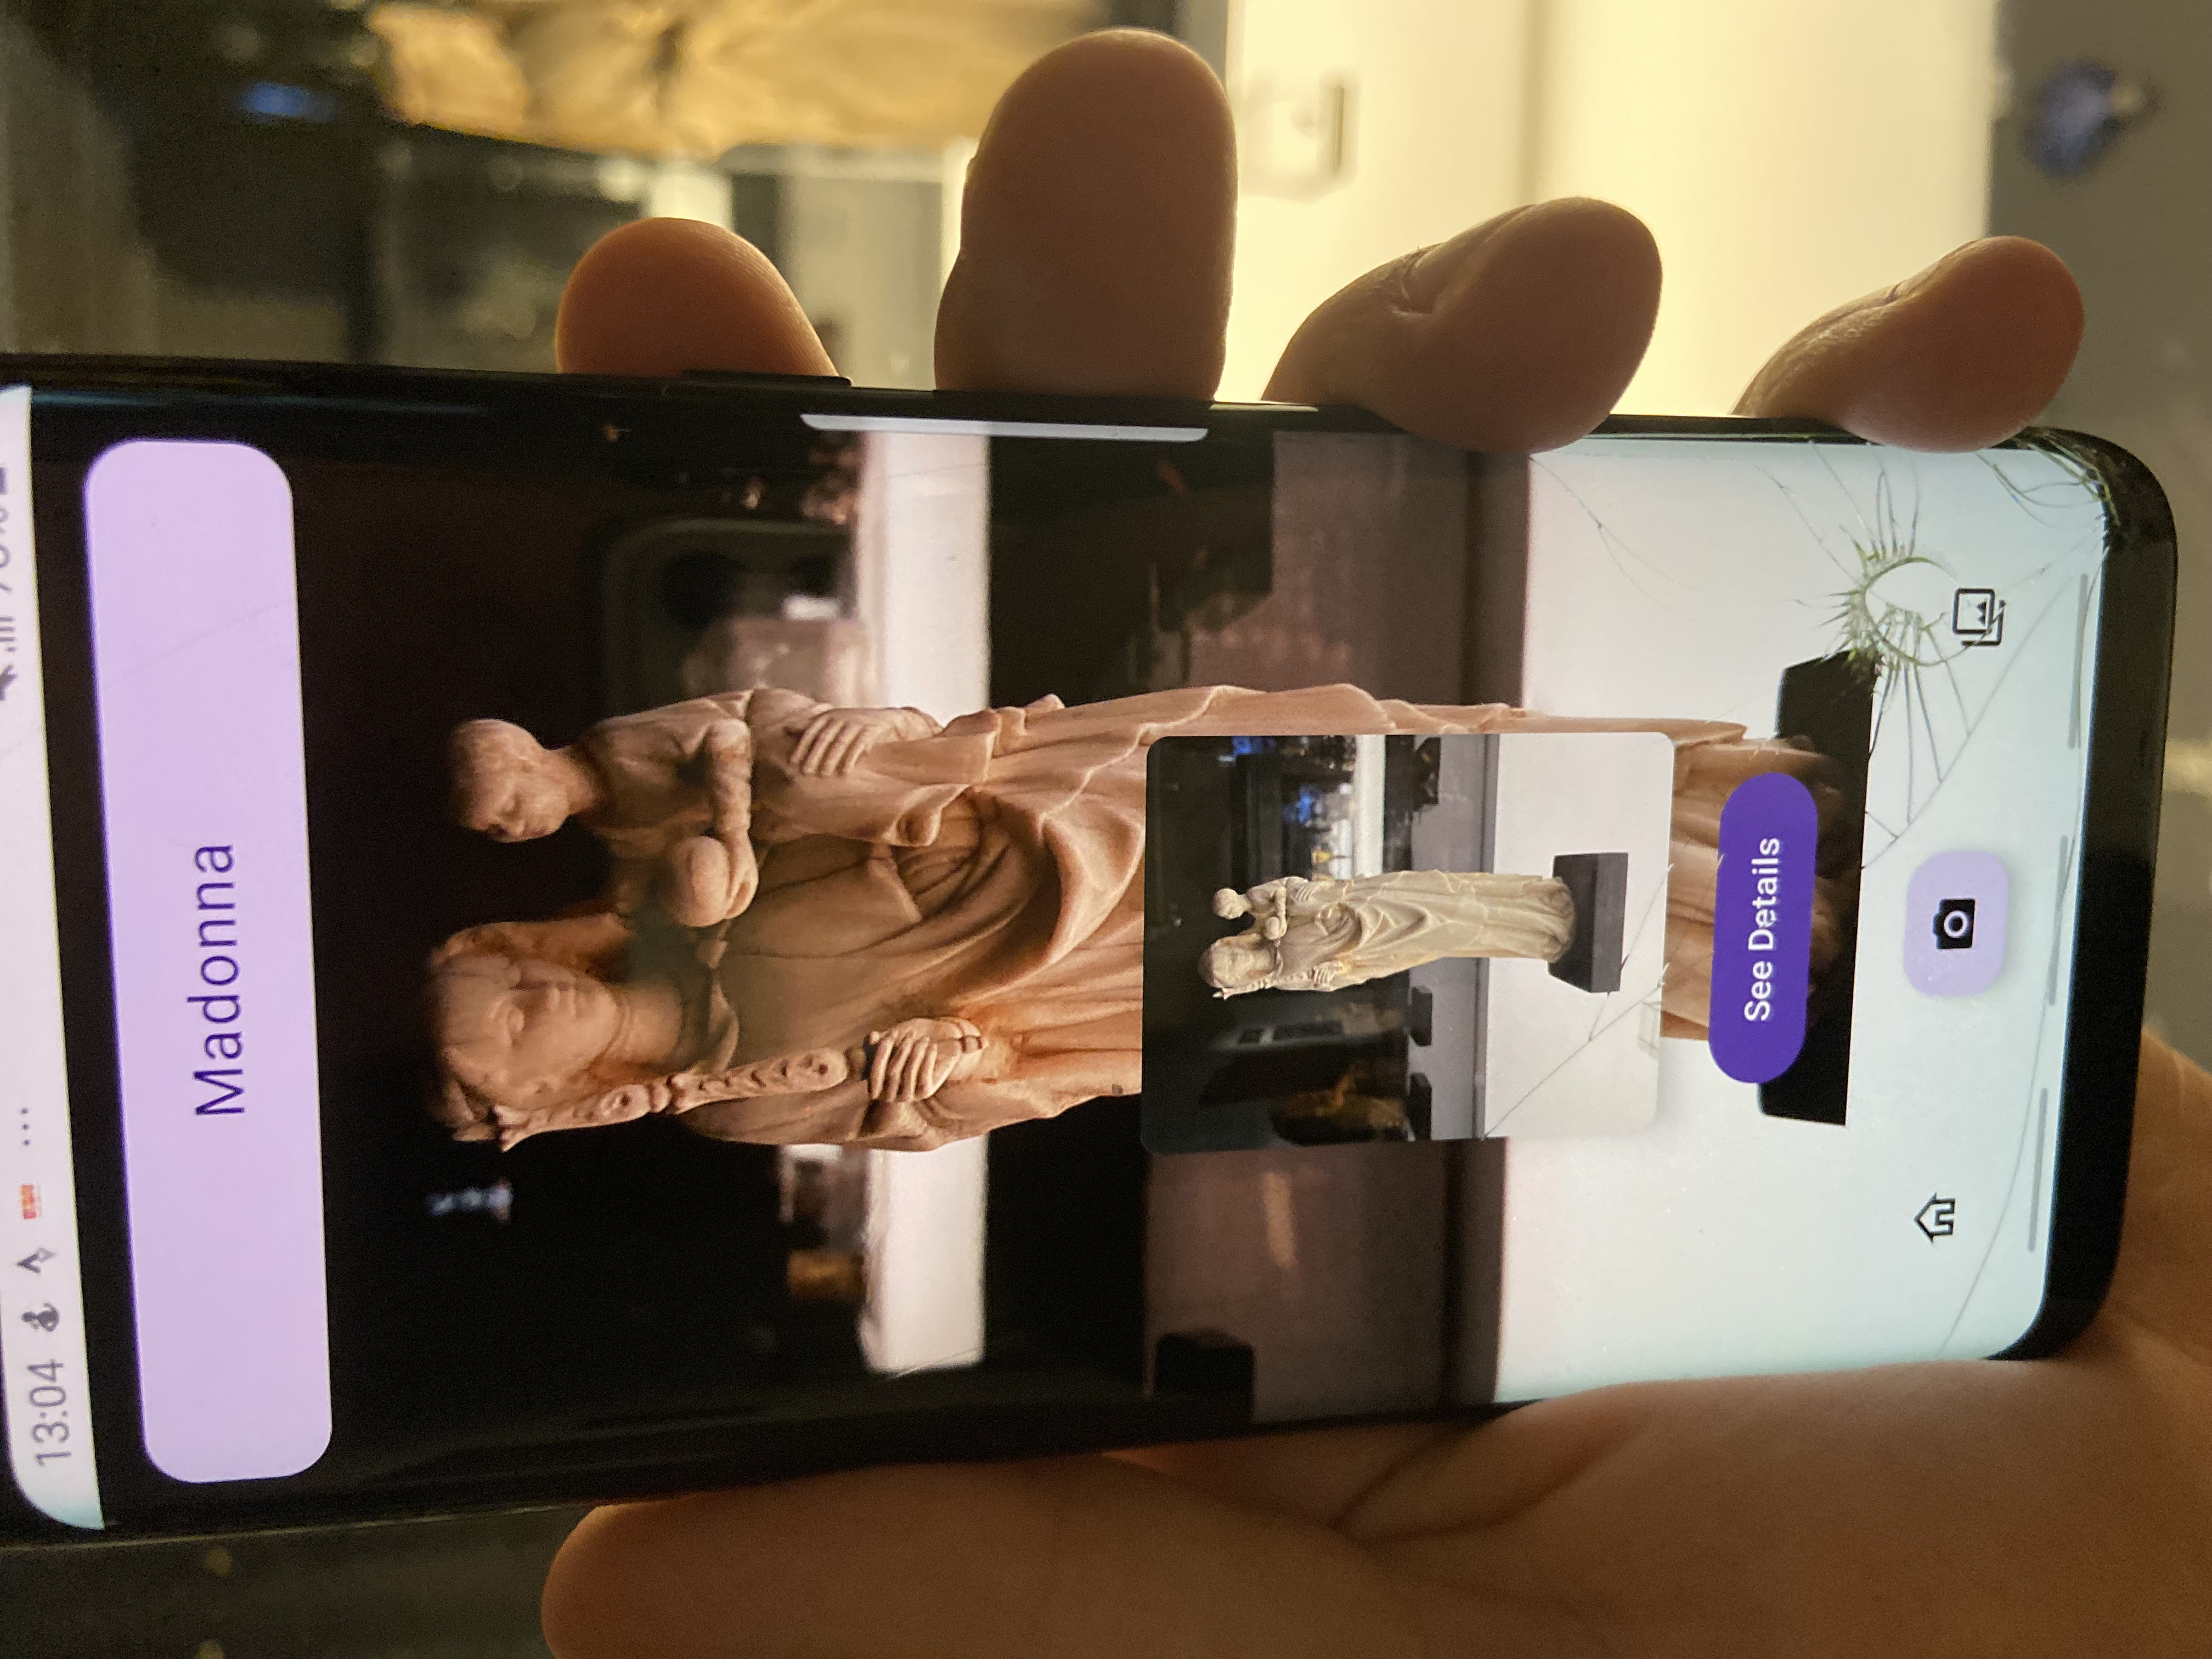
\includegraphics[angle=270, width=\textwidth]{img/test-example-4.jpg}
    \end{subfigure}

    \caption{Examples of real-world exhibit recognition.}\label{fig:test_examples}
\end{figure}

Additionally, a short video demonstrating the application during testing is available here:

\begin{center}
\url{https://www.youtube.com/shorts/eHmp9kK2hn8}
\end{center}

\section{Summary}

In summary, the developed mobile application demonstrated strong performance in real-world museum exhibit recognition, achieving a decent accuracy rate of 93.75\% on a diverse set of 80 exhibits. The application successfully identified most exhibits at the first attempt, with misclassifications being limited to visually similar items, which is a common challenge in image classification tasks. The inference time remained low, ensuring a responsive user experience, and the confidence levels of predictions were consistent with expectations. Overall, the application proved to be a valuable tool for enhancing the museum experience by providing real-time information about exhibits, confirming its practical applicability in real-world scenarios.
\chapter{User Manual}

This chapter provides instructions on how to use the mobile application effectively.

\section{Installation}

To install the application:

\begin{enumerate}
\item Transfer the provided APK file (located in the \texttt{MuseumGuideApp} folder under the name \texttt{museum-guide.apk}) to your Android smartphone.
\item Navigate to the transferred file using a file manager app.
\item Tap on the APK file to start installation. You might need to enable \textbf{Install from unknown sources} if prompted.
\item After installation, open the application from your home screen or app drawer.
\end{enumerate}

\section{Navigating the Application}

Upon launching the application, you will see the \textbf{Home Screen}, displaying general information about the museum. You can scroll down to find links to the museum's social media and contact information.

Navigate using the bottom menu with the following options:

\begin{itemize}
\item \textbf{Home}: Returns you to the Home Screen.
\item \textbf{Camera}: Opens the camera for real-time exhibit recognition.
\item \textbf{Gallery}: Displays all museum exhibits in a scrollable grid.
\end{itemize}

\section{Viewing Exhibits in Gallery}

In the \textbf{Gallery Screen}, you can scroll through and tap on any exhibit to view detailed information such as the title, author, and historical period.

\section{Real-Time Exhibit Recognition}

To use the real-time recognition feature:

\begin{enumerate}
\item Tap on the \textbf{Camera} option in the bottom menu.
\item If prompted, grant camera permissions to the application.
\item Aim your smartphone's camera at an exhibit within the museum. Recognition results will be displayed in real-time, overlaid on the camera feed.
\item Once the model recognizes an exhibit, tap \textbf{See Details} to view more information about the recognized exhibit. If the recognition is incorrect, you can check the alternatives provided below the main prediction. These alternatives are ranked by confidence level and can help you find the correct exhibit.
\end{enumerate}

\section{Debug Mode}

The application includes a Debug Mode for testing purposes:

\begin{enumerate}
\item In the \textbf{Camera Screen}, switch from \textbf{Regural} to \textbf{Debug} mode by tapping the icon in the bottom right corner.
\item Debug Mode allows you to adjust the classification confidence threshold and view detailed classification results, including confidence levels and processing time.
\end{enumerate}

To exit the Debug Mode, tap the icon again.

\chapter*{Conclusion}
\addcontentsline{toc}{chapter}{Conclusion}

In this thesis, we explored, implemented, and evaluated a mobile application capable of recognizing museum exhibits in real time. The primary objective was to provide museum visitors with quick, accurate access to information about exhibits directly through their Android smartphones.

We began by preparing a suitable dataset by recording videos of exhibits and extracting individual frames. Care was taken to ensure balanced representation of each exhibit, extracting frames at regular intervals and subsequently labeling them using metadata stored in a CSV file. This approach allowed us to create a well-structured dataset for our task.

The initial exploration of potential approaches identified two main solutions for achieving accurate image recognition: the embedding-based similarity search and direct classification using transfer learning. The first method, embedding-based similarity search, although highly flexible, was soon discarded due to practical limitations, notably the high computational requirements and significant storage overhead of embeddings on mobile devices. Alternatively, direct classification through transfer learning proved to be the most suitable option, balancing accuracy, performance, ease of integration, and storage efficiency.

For the classification architecture, MobileNetV2 was chosen due to its compact and efficient design aimed at mobile environments. Through experimentation with different configurations --- such as batch sizes, number of layers, dropout rates, and fine-tuning --- we arrived at a final optimized model that achieved validation accuracy of approximately 95.9\%.

An analysis of misclassifications revealed that errors mostly occurred on visually similar exhibits or when multiple objects appeared within a single image. To mitigate this, the application's user interface includes not only the model's top prediction but also several alternative suggestions (in a non-intrusive manner). This allows users to easily access information about exhibits, even when predictions are not entirely accurate.

The developed Android application integrates TensorFlow Lite for lightweight on-device inference and employs CameraX for simple, efficient camera access. The application includes multiple screens --- from a home and gallery view to dedicated exhibit detail and real-time scanner screens --- organized clearly and intuitively. Additionally, a debug mode was implemented for convenient monitoring and adjusting classification thresholds and inference time evaluation.

Real-world testing was conducted at the Museum of Decorative Arts in Prague (UPM). Practical evaluation on a subset of 80 museum exhibits yielded an accuracy of around 93.75\%, closely matching expectations derived from validation results. Misclassifications again typically involved visually similar exhibits, yet the correct exhibit usually appeared within the offered alternative suggestions. Furthermore, inference was fast enough --- around 120--150 ms --- to provide smooth, responsive real-time interaction.

Nevertheless, there are several practical ways to build upon this work. Expanding the dataset is always beneficial, as training on more images under various conditions generally helps models achieve better generalization. Additionally, future work could explore alternative neural network architectures apart from MobileNetV2; examples include EfficientNet Lite or ShuffleNet, both specifically designed to run efficiently on mobile devices while maintaining good classification accuracy. It could also be beneficial to experiment with entirely different approaches, including object detection techniques such as YOLO or SSD. Object detection would enable simultaneous localization and recognition of multiple exhibits within a single camera frame, directly addressing one of the challenges identified during evaluation. Furthermore, hybrid approaches that combine CNN-based models with classical image descriptors or utilize additional sensor data (e.g., Bluetooth beacons or NFC tags) could offer increased robustness and improved recognition performance in challenging scenarios.

Overall, this work successfully demonstrated that modern machine learning methods in combination with optimized model architectures and mobile technologies can effectively support real-time museum exhibit recognition. The resulting application not only performed reliably within a controlled evaluation but also showed potential applicability to broader museum contexts. With incremental improvements and adaptations, such tools could meaningfully assist visitors, providing convenient, immediate, and easy-to-access information right at their fingertips.


%%% Bibliography
%%% Bibliography (literature used as a source)
%%%
%%% We employ biblatex to construct the bibliography. It processes
%%% citations in the text (e.g., the \cite{...} macro) and looks up
%%% relevant entries in the bibliography.bib file.
%%%
%%% See also biblatex settings in thesis.tex.

%%% Generate the bibliography. Beware that if you cited no works,
%%% the empty list will be omitted completely.

% We let bibliography items stick out of the right margin a little
\def\bibfont{\hfuzz=2pt}

\printbibliography[heading=bibintoc]

%%% If case you prefer to write the bibliography manually (without biblatex),
%%% you can use the following. Please follow the ISO 690 standard and
%%% citation conventions of your field of research.

% \begin{thebibliography}{99}
%
% \bibitem{lamport94}
%   {\sc Lamport,} Leslie.
%   \emph{\LaTeX: A Document Preparation System}.
%   2nd edition.
%   Massachusetts: Addison Wesley, 1994.
%   ISBN 0-201-52983-1.
%
% \end{thebibliography}


%%% Figures used in the thesis (consider if this is needed)
\listoffigures

%%% Tables used in the thesis (consider if this is needed)
%%% In mathematical theses, it could be better to move the list of tables to the beginning of the thesis.
\listoftables

%%% Abbreviations used in the thesis, if any, including their explanation
%%% In mathematical theses, it could be better to move the list of abbreviations to the beginning of the thesis.
% \chapwithtoc{List of Abbreviations}

%%% Doctoral theses must contain a list of author's publications
\ifx\ThesisType\TypePhD
\chapwithtoc{List of Publications}
\fi

%%% Attachments to the thesis, if any. Each attachment must be referred to
%%% at least once from the text of the thesis. Attachments are numbered.
%%%
%%% The printed version should preferably contain attachments, which can be
%%% read (additional tables and charts, supplementary text, examples of
%%% program output, etc.). The electronic version is more suited for attachments
%%% which will likely be used in an electronic form rather than read (program
%%% source code, data files, interactive charts, etc.). Electronic attachments
%%% should be uploaded to SIS. Allowed file formats are specified in provision
%%% of the rector no. 72/2017. Exceptions can be approved by faculty's coordinator.
% \appendix
% \chapter{Attachments}

% \section{First Attachment}

\end{document}
